\chapter{Results and Analysis} \label{ch:results-analysis}

We demonstrate the output of the Frangi filter on our samples after running a multiscale technique with $N=20$ scales with a stricter anisotropy parameter $\beta = 0.35$ and standard structureness parameter $\gamma=0.5$,
with scales spaced logarithmically from $\sigma_1 = 2^{-1}$ to $\sigma_N = 2^{3.5}$, performing glare and cut removal in preprocessing, and using a discrete gaussian kernel and dilation border of 20.
Our goal in this section is to provide a close up look at the Frangi filter on two samples, and then provide some measures of the Frangi output's correspondence with the ``ground truth'' network tracings across all 201 images, without explicitly performing segmentation. However, for visual demonstration, we will employ both simple thresholding techniques (arbitrary fixed and nonzero-percentile) described in \cref{ch:multifrangi}. In \cref{ch:segmentation} we will develop and analyze more sophisticated Frangi-based segmentation techniques and compare their performance to these rudimentary thresholding techniques across the entire dataset. For this chapter we will content ourselves with analysis of the raw Frangi vesselness measure within our image domain, and use our simple thresholded results for visual demonstration alone.

\section{Sample visual output}
In \cref{fig:detailed_output_with_table_ex1} and \cref{fig:detailed_frangi_with_table_ex2} we take a look at the Frangi output (\Vmax) for a well-behaved sample. In the left column we have (from top to bottom) the un-preprocessed placental sample, the preprocessed sample, the color trace(ground truth), and $\Vmax$. In the top-right, we have for each $n=0,...,19$ scales, we have the size of the scale $\sigma_n$, the 95th percentile score at that scale  $\alpha_p$ where $p=95$, and the maximum vesselness score at that scale ($\max(V_\sigma)$. The bottom-right set of images are two rudimentary thresholds of the Frangi result. The top is the scalewise nonzero percentile threshold (95th percentile) and the bottom is a strict threshold of 0.4. left and right images are two rudimentary thresholds of $\Vmax$. The bottom left is nonzero percentile filtering (thresholded at the 95th percentile, and the  right image is a simple threshold at $\alpha=0.4$. For each pixel that passes the threshold, each of these graphs is color coded to indicate from which scale the maximum value at that pixel occurs, colored according to the scale on the left. These two thresholds are included mostly to further show the dependence of scale on which vessels are identified.
% these montages were manually stitched together from
% 181127-sievetest

%\begin{figure} \centering
%  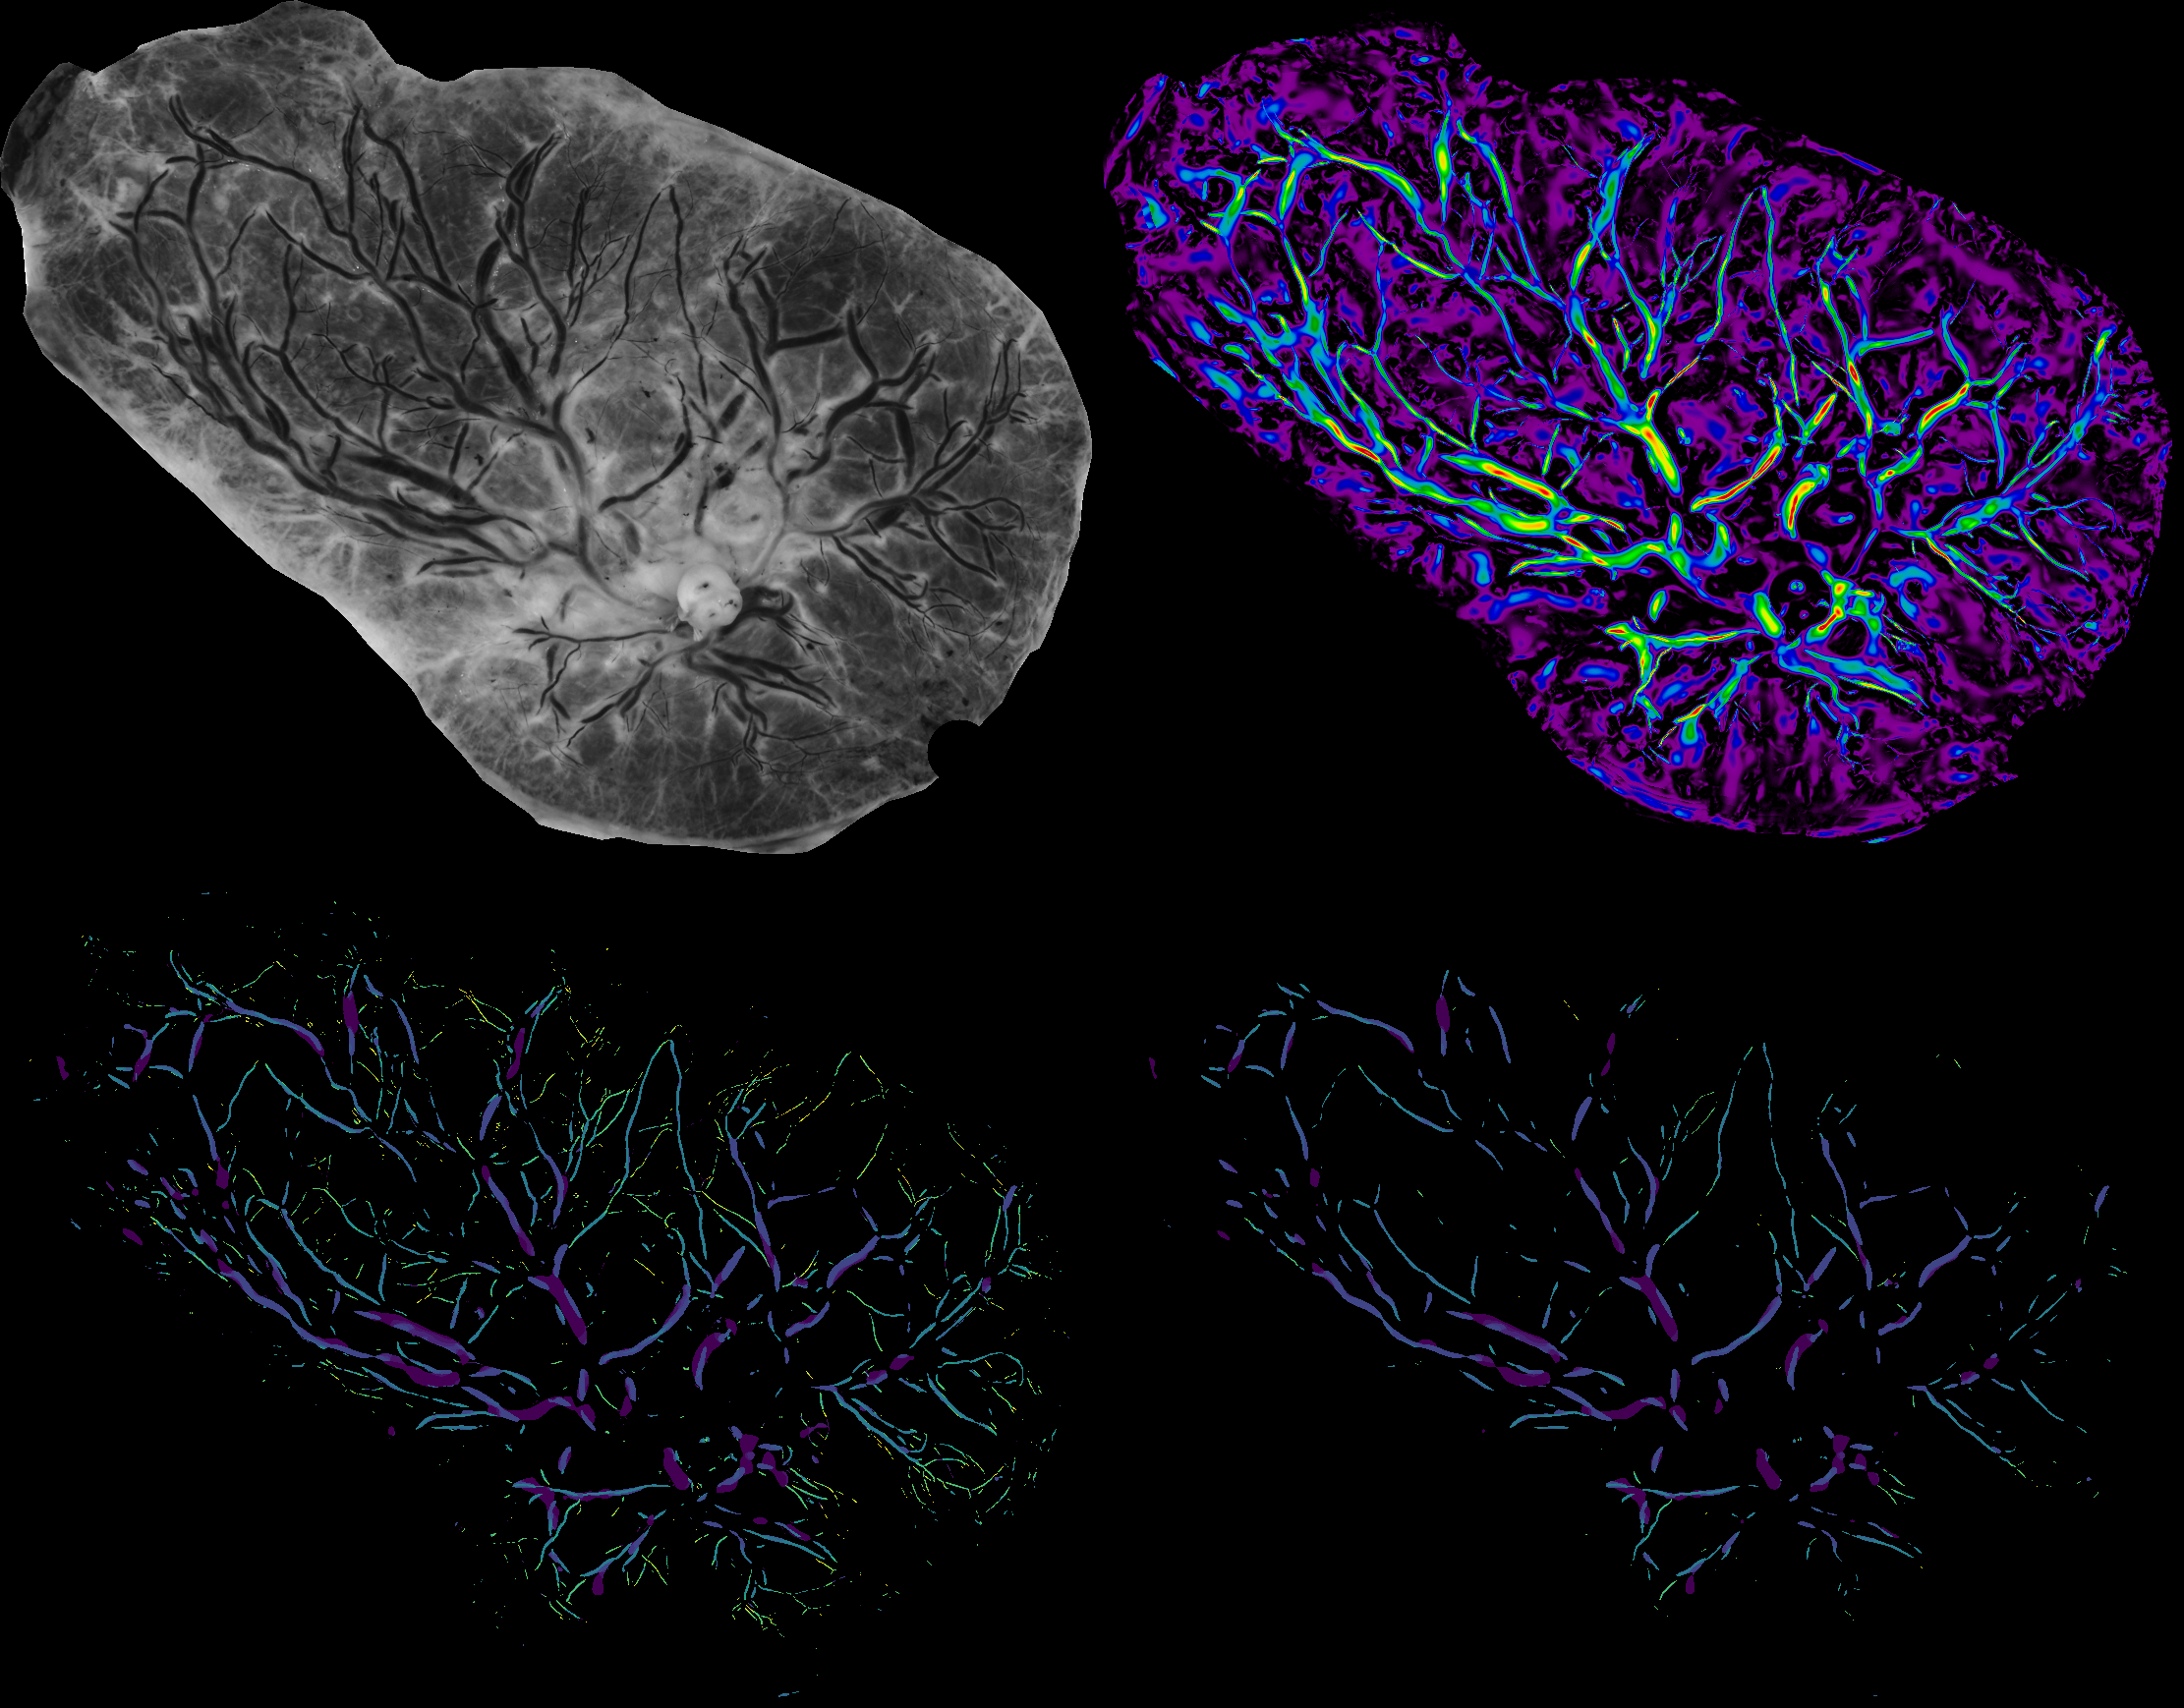
\includegraphics[width=\textwidth]{montage-T-BN0164923}
%  \caption{Sample Multiscale Frangi output ($\beta=0.35$) with simple segmentation strategies (Example 1)}
%  \label{fig:output-montage-example1}
%\end{figure}
%
%\begin{figure} \centering
%  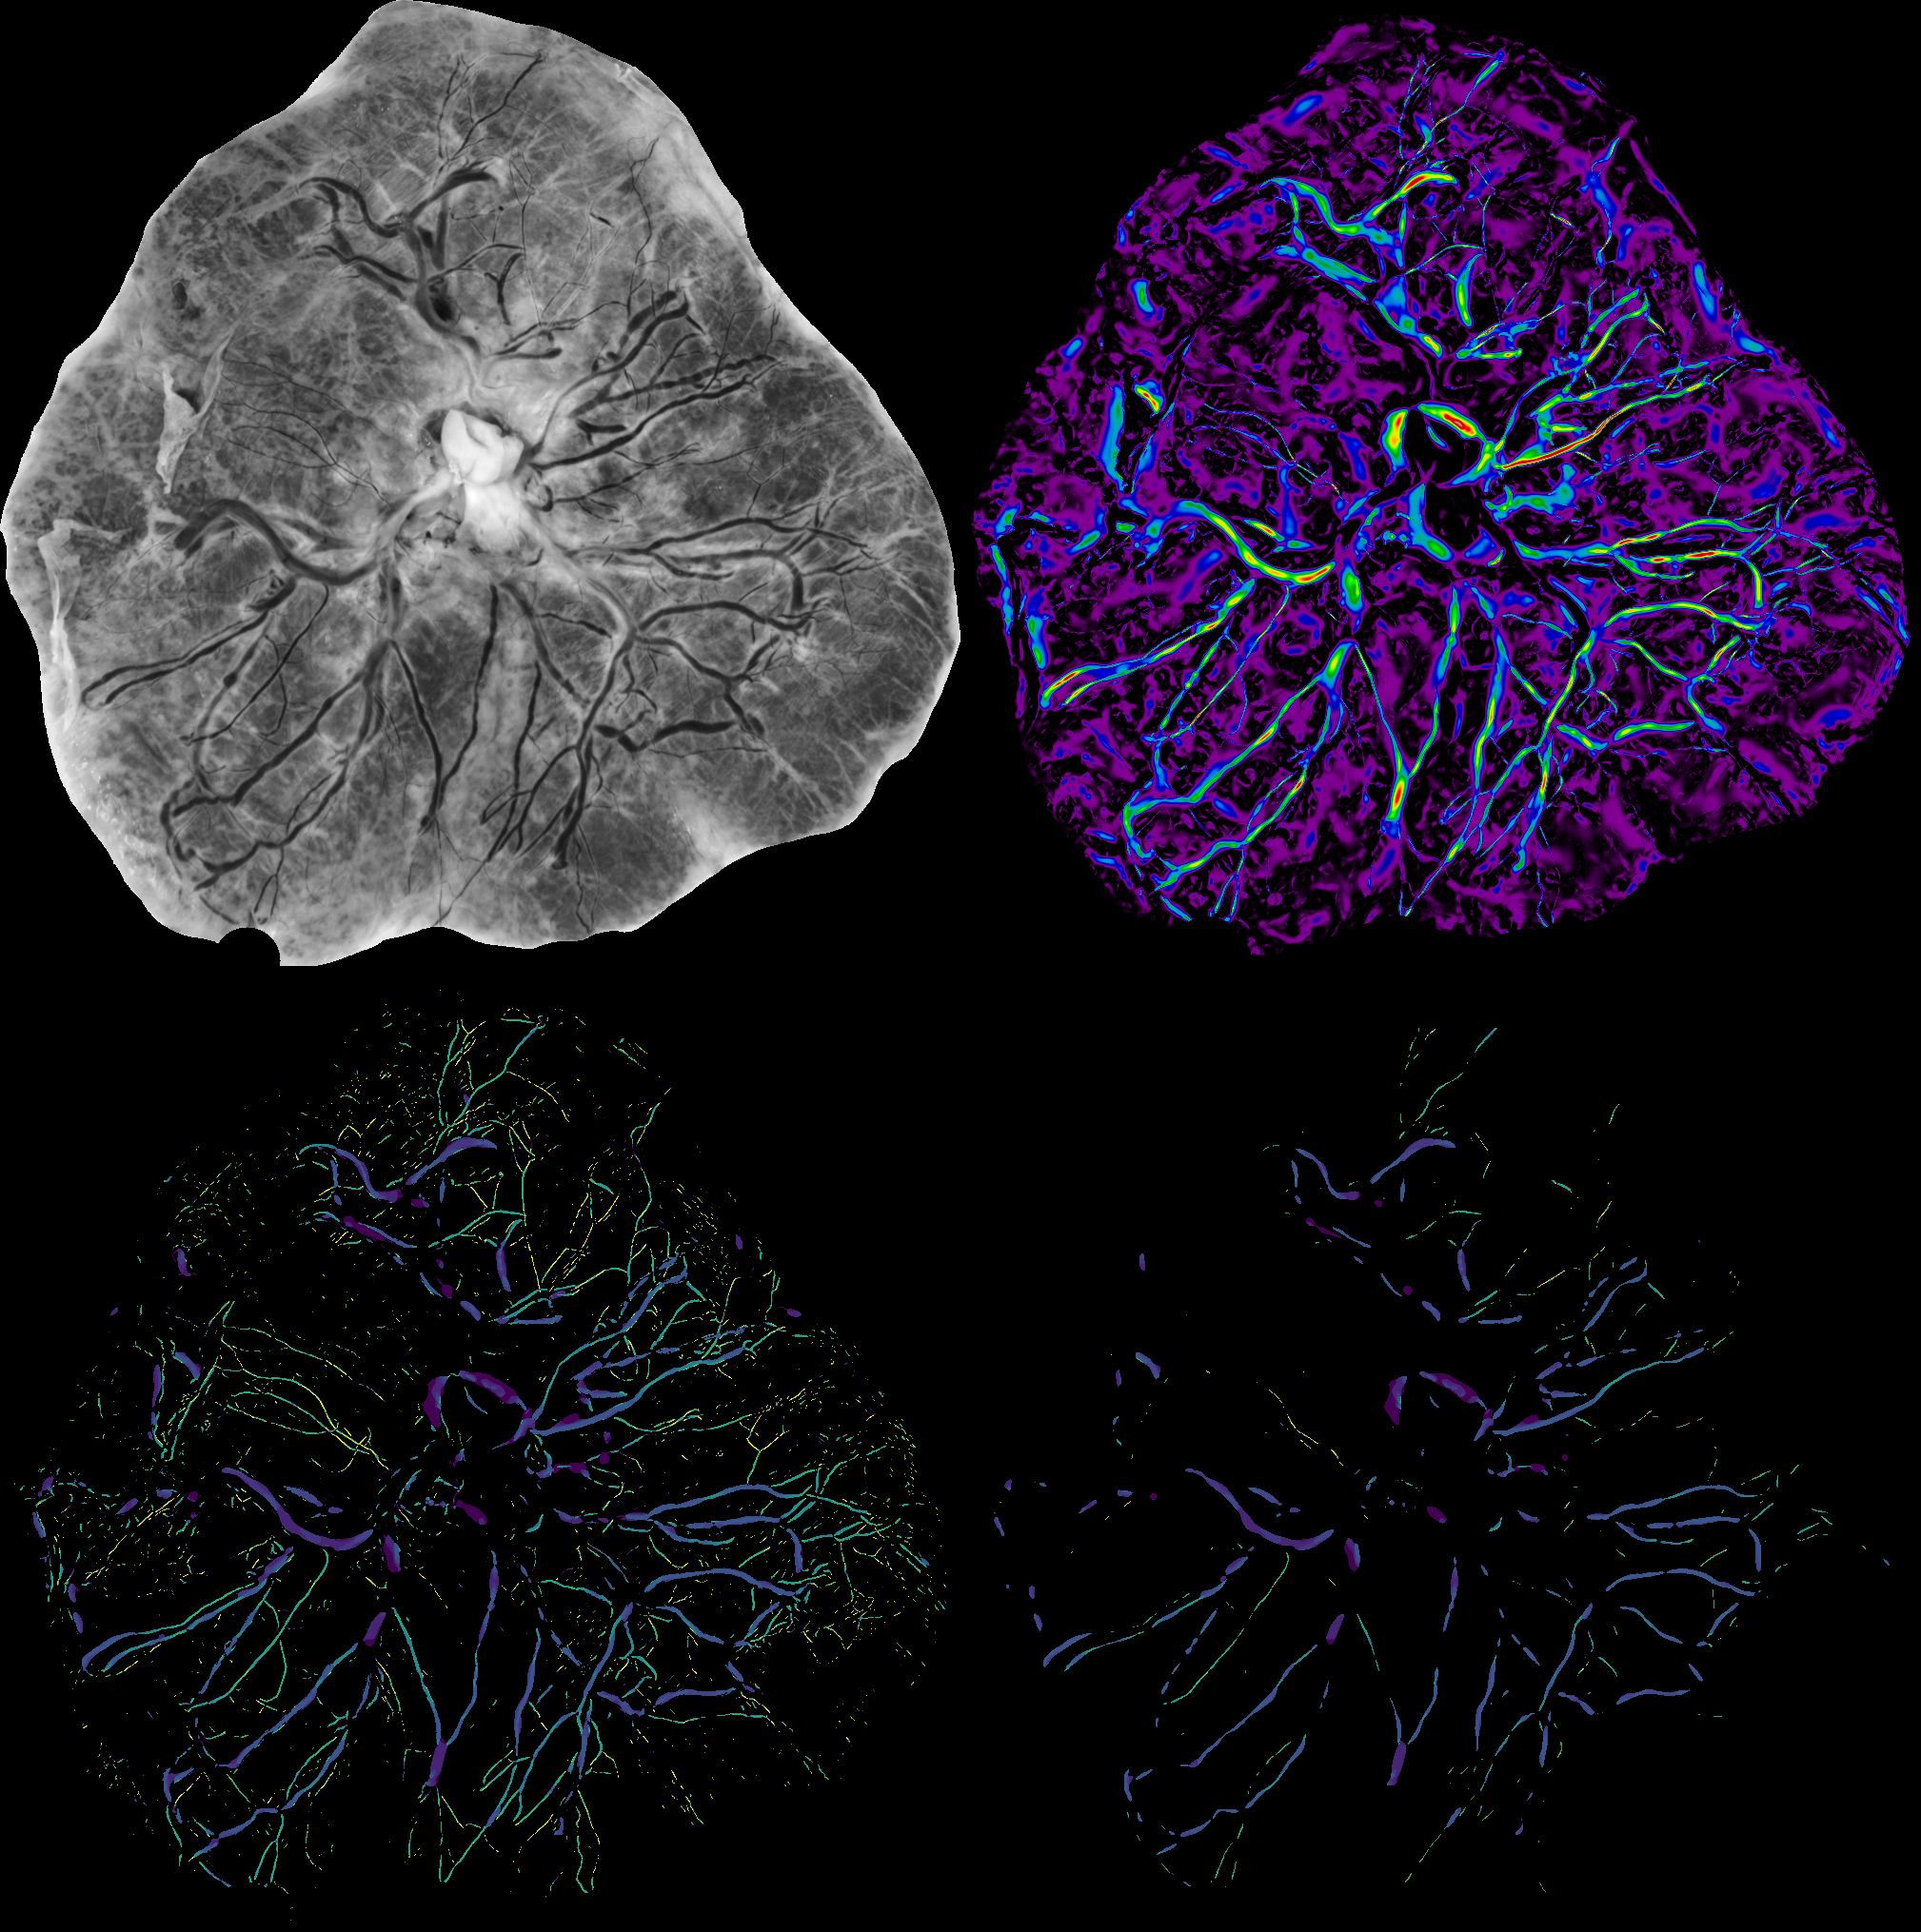
\includegraphics[width=\textwidth]{montage-T-BN0651415}
%  \caption{Sample Multiscale Frangi output ($\beta=0.35$) with simple segmentation strategies (Example 2)}
%  \label{fig:output-montage-example2}
%\end{figure}

\begin{figure}
  \begin{minipage}[tp]{0.5\textwidth}
    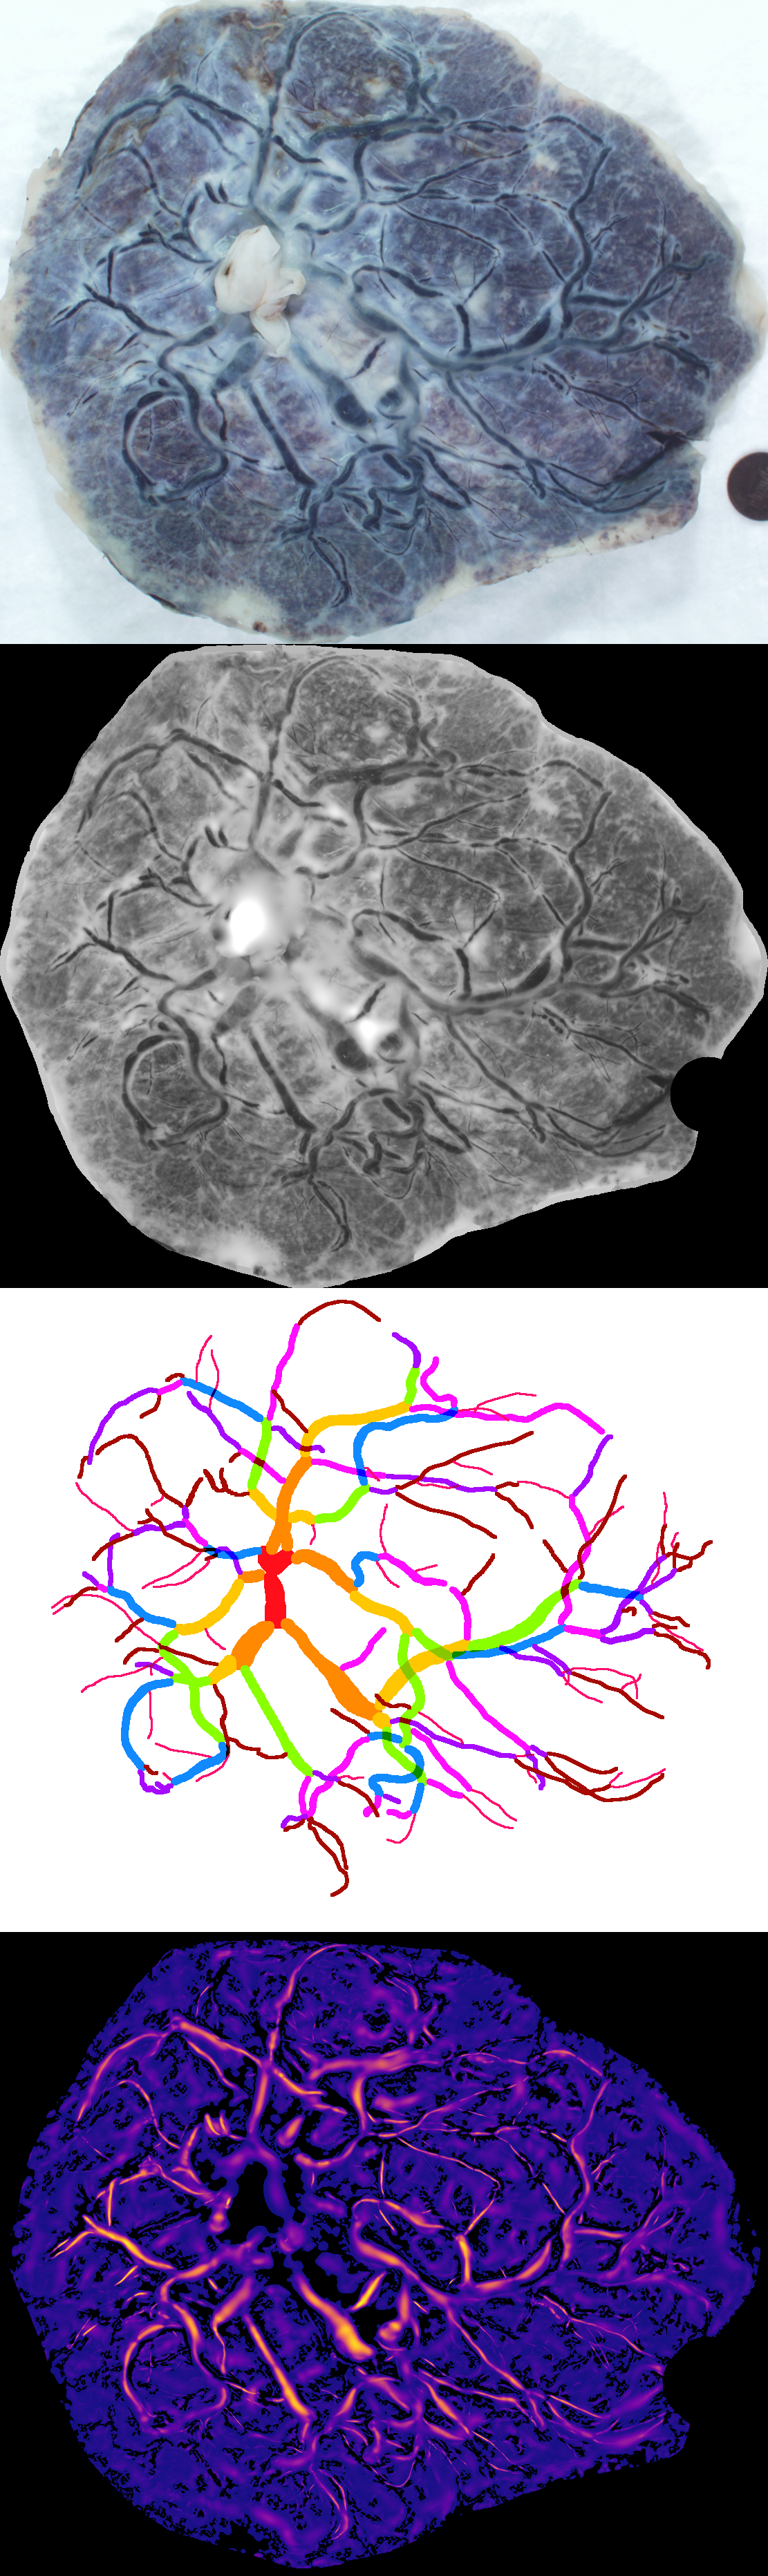
\includegraphics[height=0.95\textheight]{M1-T-BN2050224}
  \end{minipage}
  \begin{minipage}[tp]{0.5\textwidth}
    \begin{tabular}{r|c|c|c}
      n  & $\sigma_n$  &  $\alpha_p$  &  $\max(V_\sigma)$ \\
      \hline
      0  &   0.353 &  0.054 &  0.986\\
      1  &   0.424 &  0.059 &  0.979\\
      2  &   0.509 &  0.065 &  0.970\\
      3  &   0.611 &  0.076 &  0.973\\
      4  &   0.733 &  0.089 &  0.988\\
      5  &   0.880 &  0.096 &  0.991\\
      6  &   1.056 &  0.108 &  0.991\\
      7  &   1.267 &  0.130 &  0.970\\
      8  &   1.521 &  0.166 &  0.973\\
      9  &   1.825 &  0.223 &  0.978\\
      10 &   2.190 &  0.292 &  0.984\\
      11 &   2.629 &  0.319 &  0.968\\
      12 &   3.155 &  0.326 &  0.994\\
      13 &   3.786 &  0.355 &  0.998\\
      14 &   4.544 &  0.405 &  0.999\\
      15 &   5.454 &  0.376 &  0.963\\
      16 &   6.545 &  0.318 &  0.950\\
      17 &   7.855 &  0.304 &  0.958\\
      18 &   9.427 &  0.328 &  0.916\\
      19 &  11.313 &  0.352 &  0.916\\
    \end{tabular} \\
    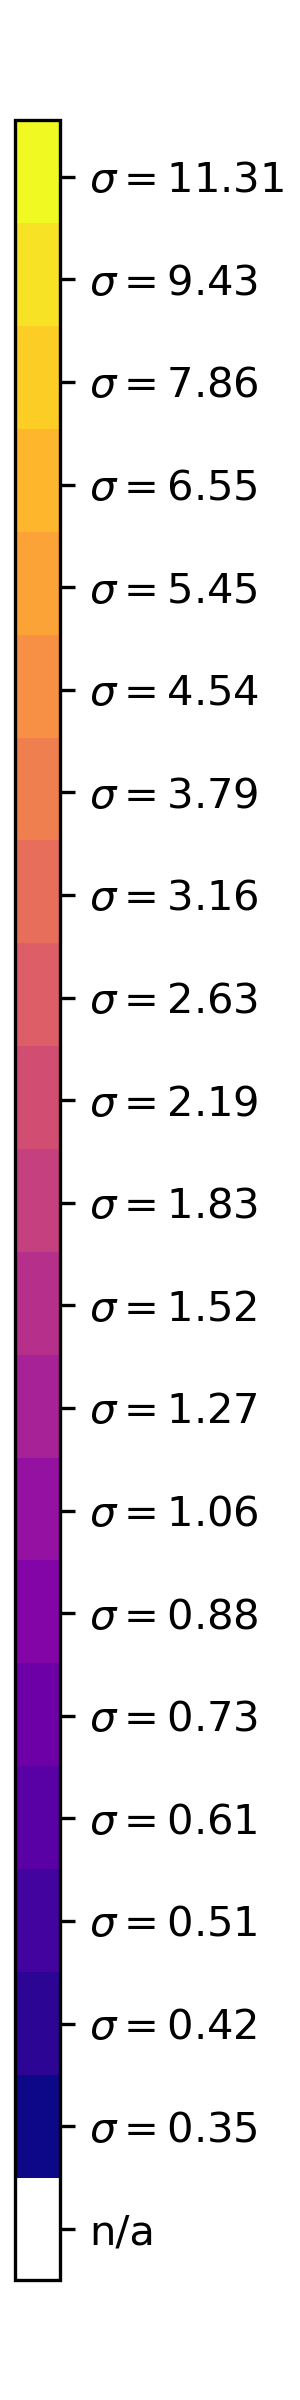
\includegraphics[height=0.5\textheight]{scale_colorbar-plasma} \;
    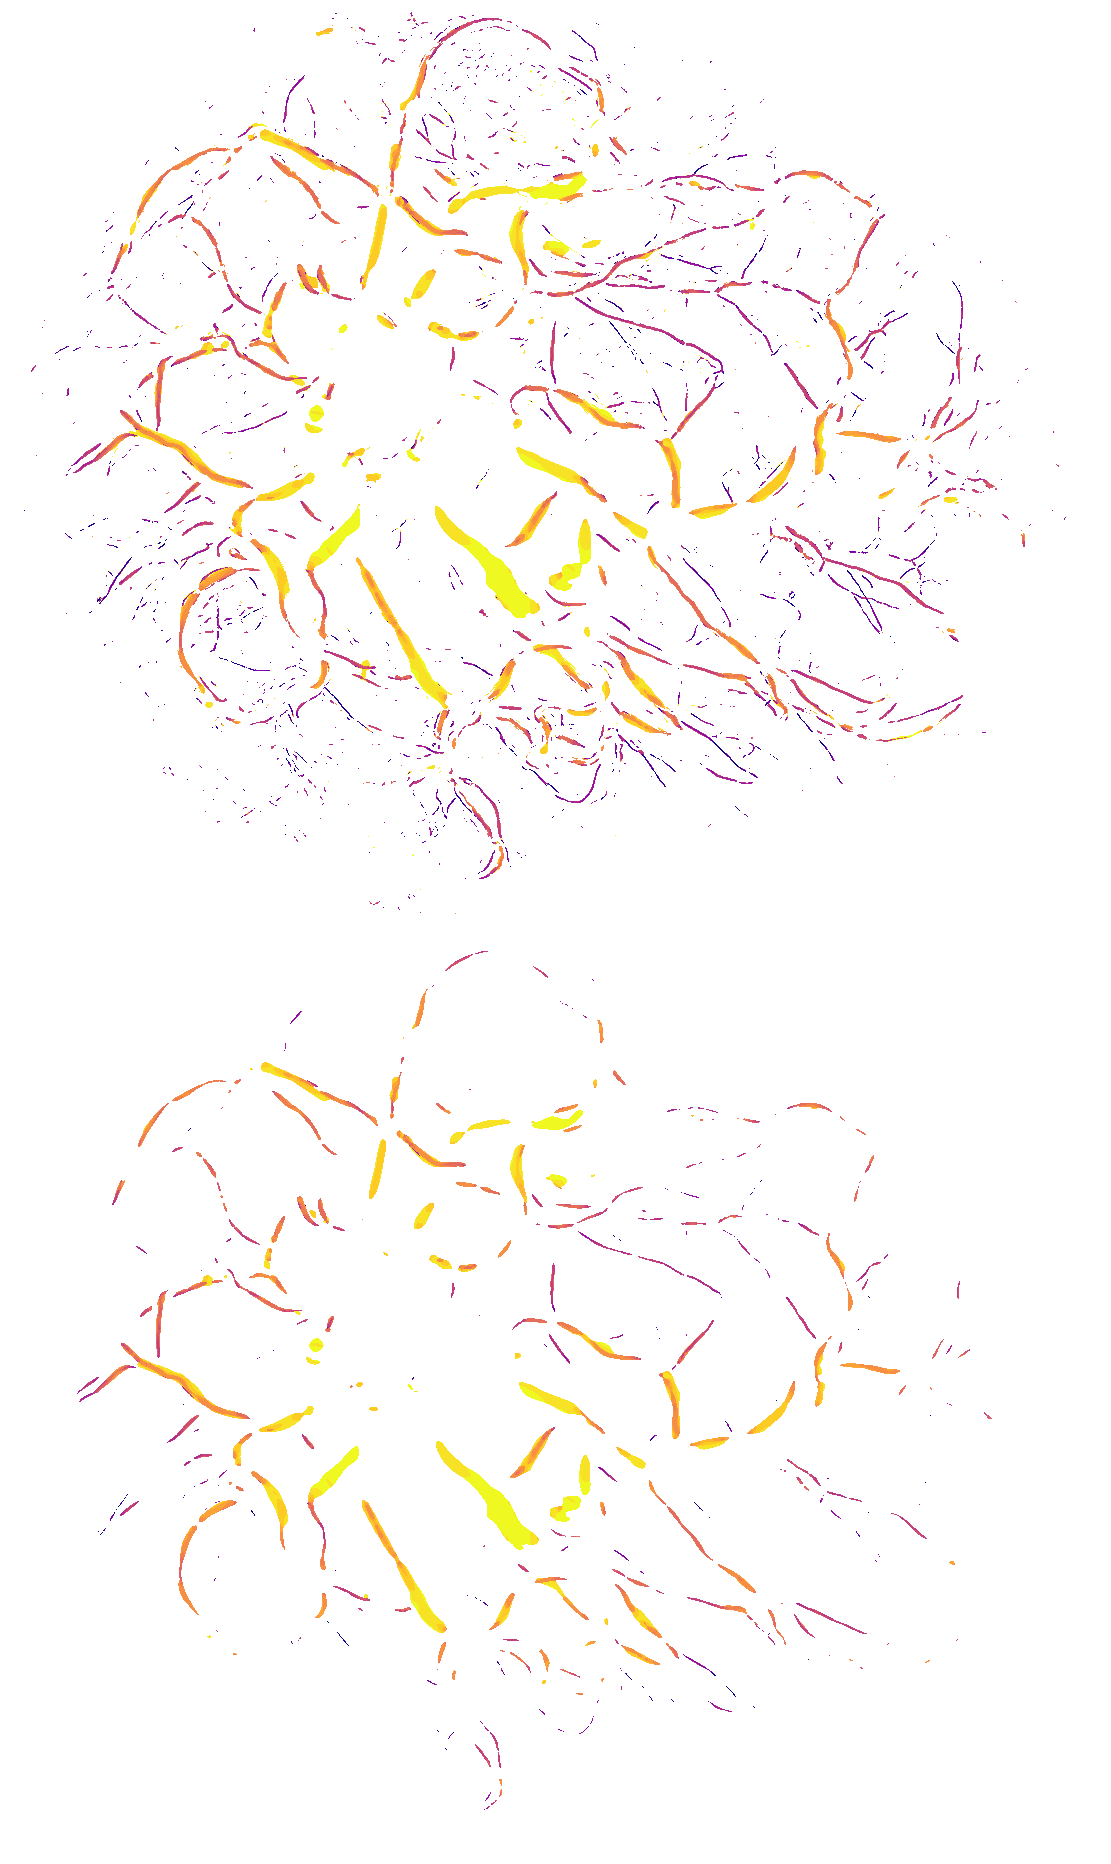
\includegraphics[height=0.5\textheight]{T-BN2050224-simple_thresholds}
  \end{minipage}
  \caption{Vesselness score, percentile thresholds, and simple thresholds,  Example 1}
  \label{fig:detailed_output_with_table_ex1}
\end{figure}

\begin{figure}
  \begin{minipage}[tp]{0.5\textwidth}
    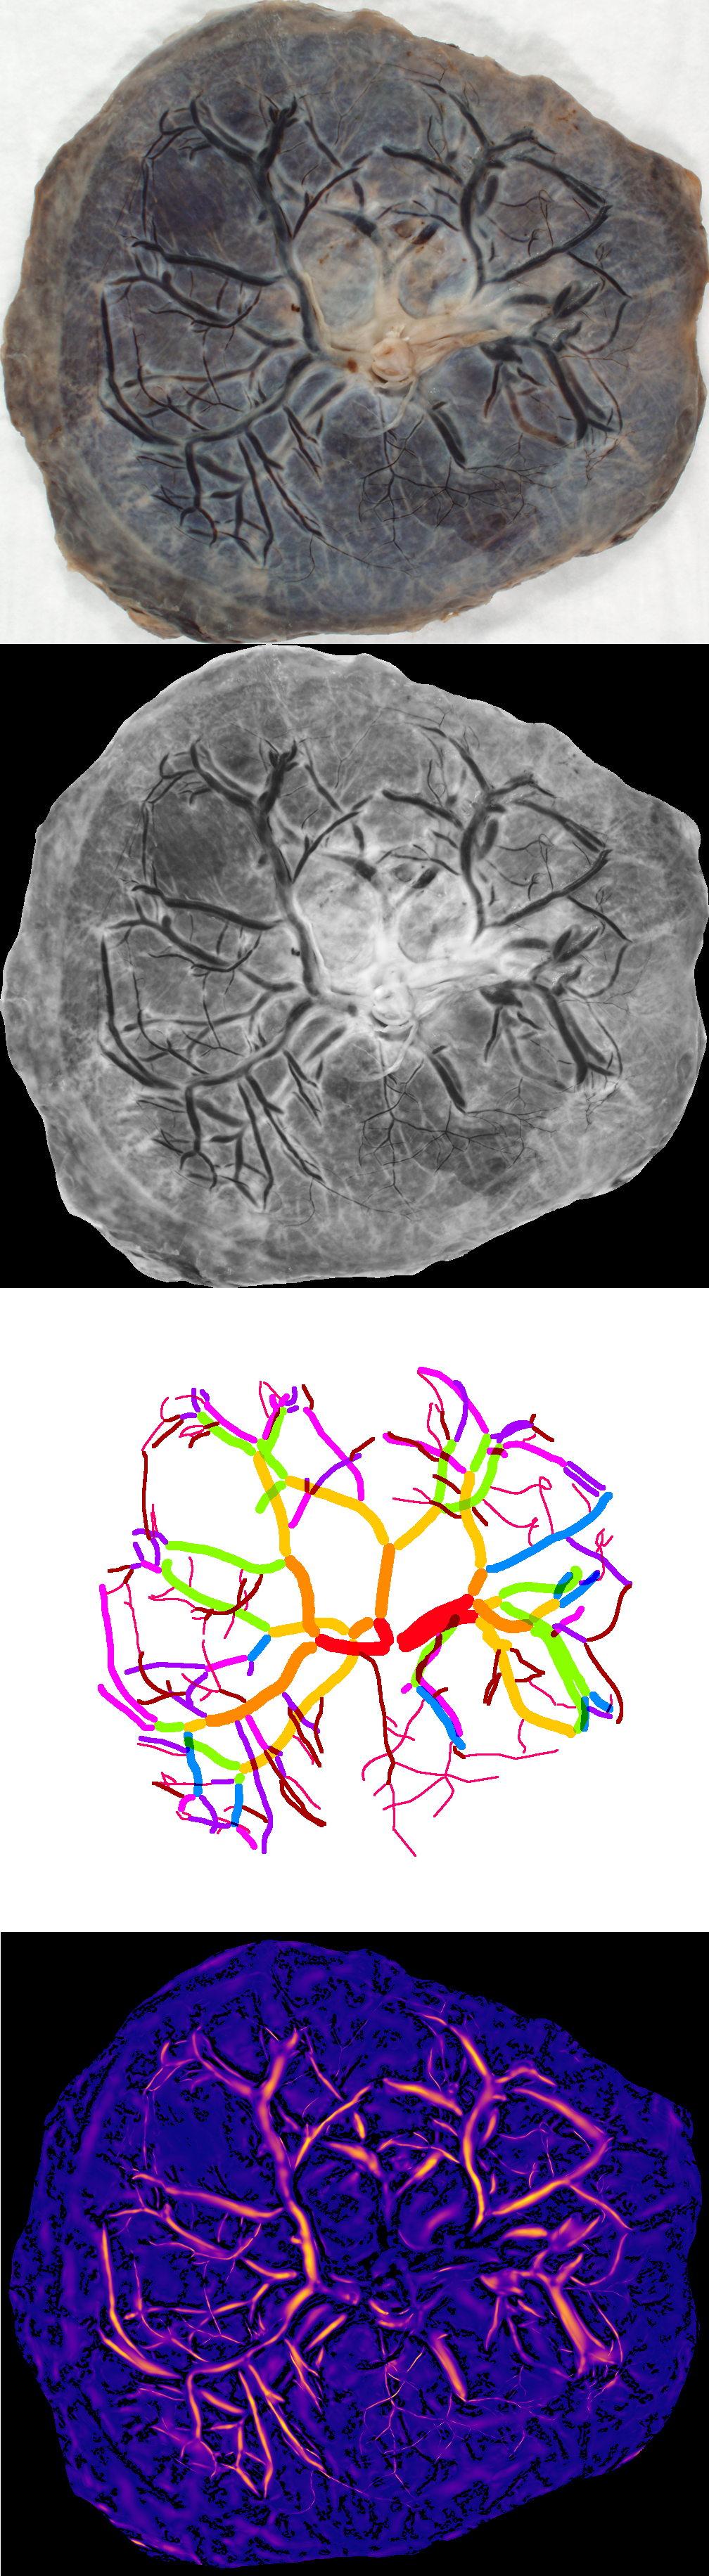
\includegraphics[height=0.95\textheight]{M1-T-BN5280796}
  \end{minipage}
  \begin{minipage}[tp]{0.5\textwidth}
    \begin{tabular}{r|c|c|c}
      $n$  & $\sigma_n$  &  $\alpha_p$  &  $\max(V_\sigma)$ \\
      \hline
      0  &  0.353 &  0.054 &  0.999 \\
      1  &  0.424 &  0.059 &  0.999 \\
      2  &  0.509 &  0.065 &  0.999 \\
      3  &  0.611 &  0.076 &  0.999 \\
      4  &  0.733 &  0.089 &  0.999 \\
      5  &  0.880 &  0.096 &  0.981 \\
      6  &  1.056 &  0.108 &  0.916 \\
      7  &  1.267 &  0.130 &  0.889 \\
      8  &  1.521 &  0.166 &  0.917 \\
      9  &  1.825 &  0.223 &  0.938 \\
      10 &  2.190 &  0.292 &  0.935 \\
      11 &  2.629 &  0.319 &  0.961 \\
      12 &  3.155 &  0.326 &  0.987 \\
      13 &  3.786 &  0.355 &  0.987 \\
      14 &  4.544 &  0.405 &  0.971 \\
      15 &  5.454 &  0.376 &  0.991 \\
      16 &  6.545 &  0.318 &  0.888 \\
      17 &  7.855 &  0.304 &  0.876 \\
      18 &  9.427 &  0.328 &  0.930 \\
      19 & 11.313 &  0.352 &  0.900 \\
    \end{tabular} \\           
    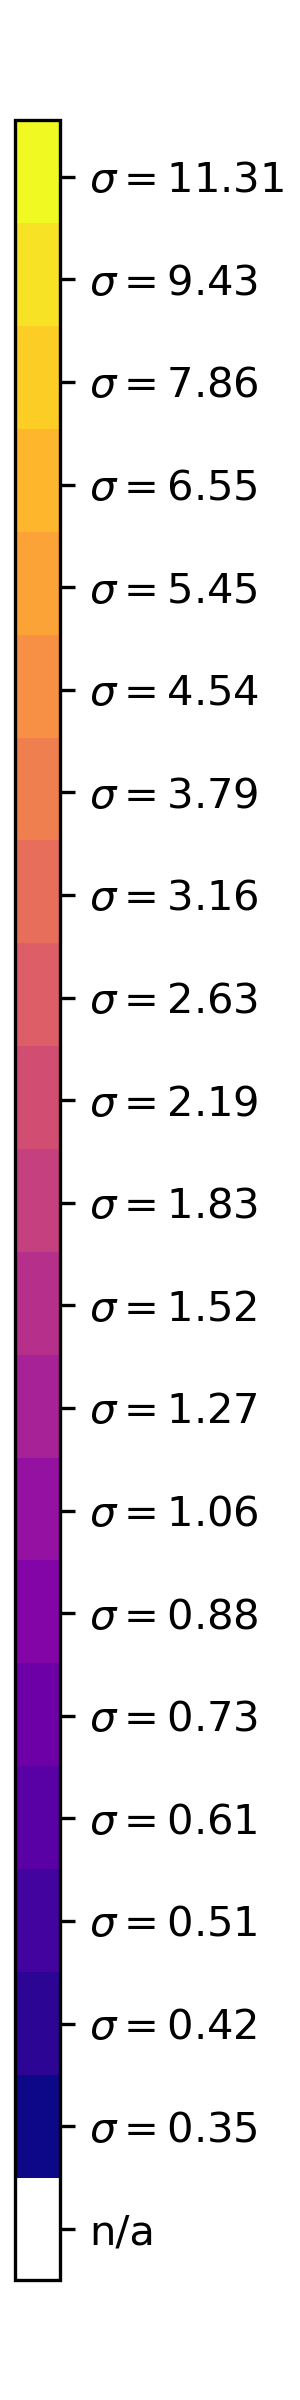
\includegraphics[height=0.5\textheight]{scale_colorbar-plasma} \;
    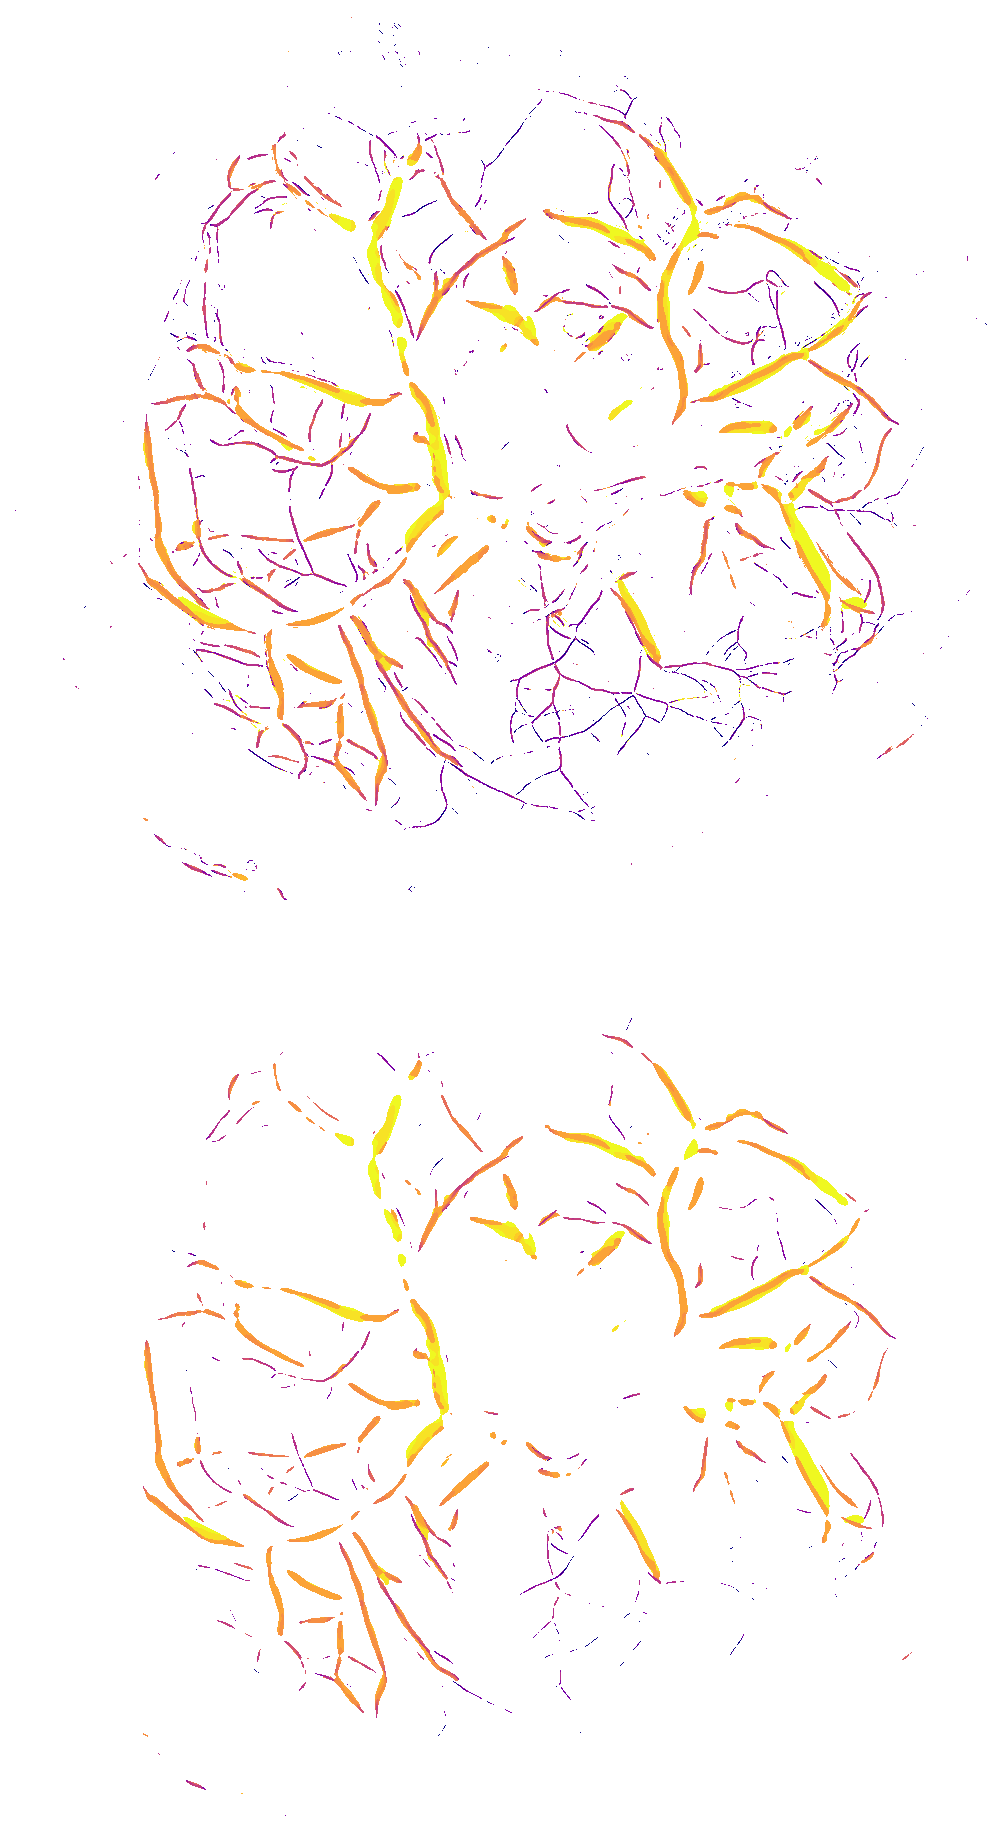
\includegraphics[height=0.5\textheight]{T-BN5280796-simple_thresholds}
  \end{minipage}
  \caption{Vesselness score, percentile thresholds, and simple thresholds, Example 2}
  \label{fig:detailed_frangi_with_table_ex2}
\end{figure}


%\begin{figure}[p] \centering
%	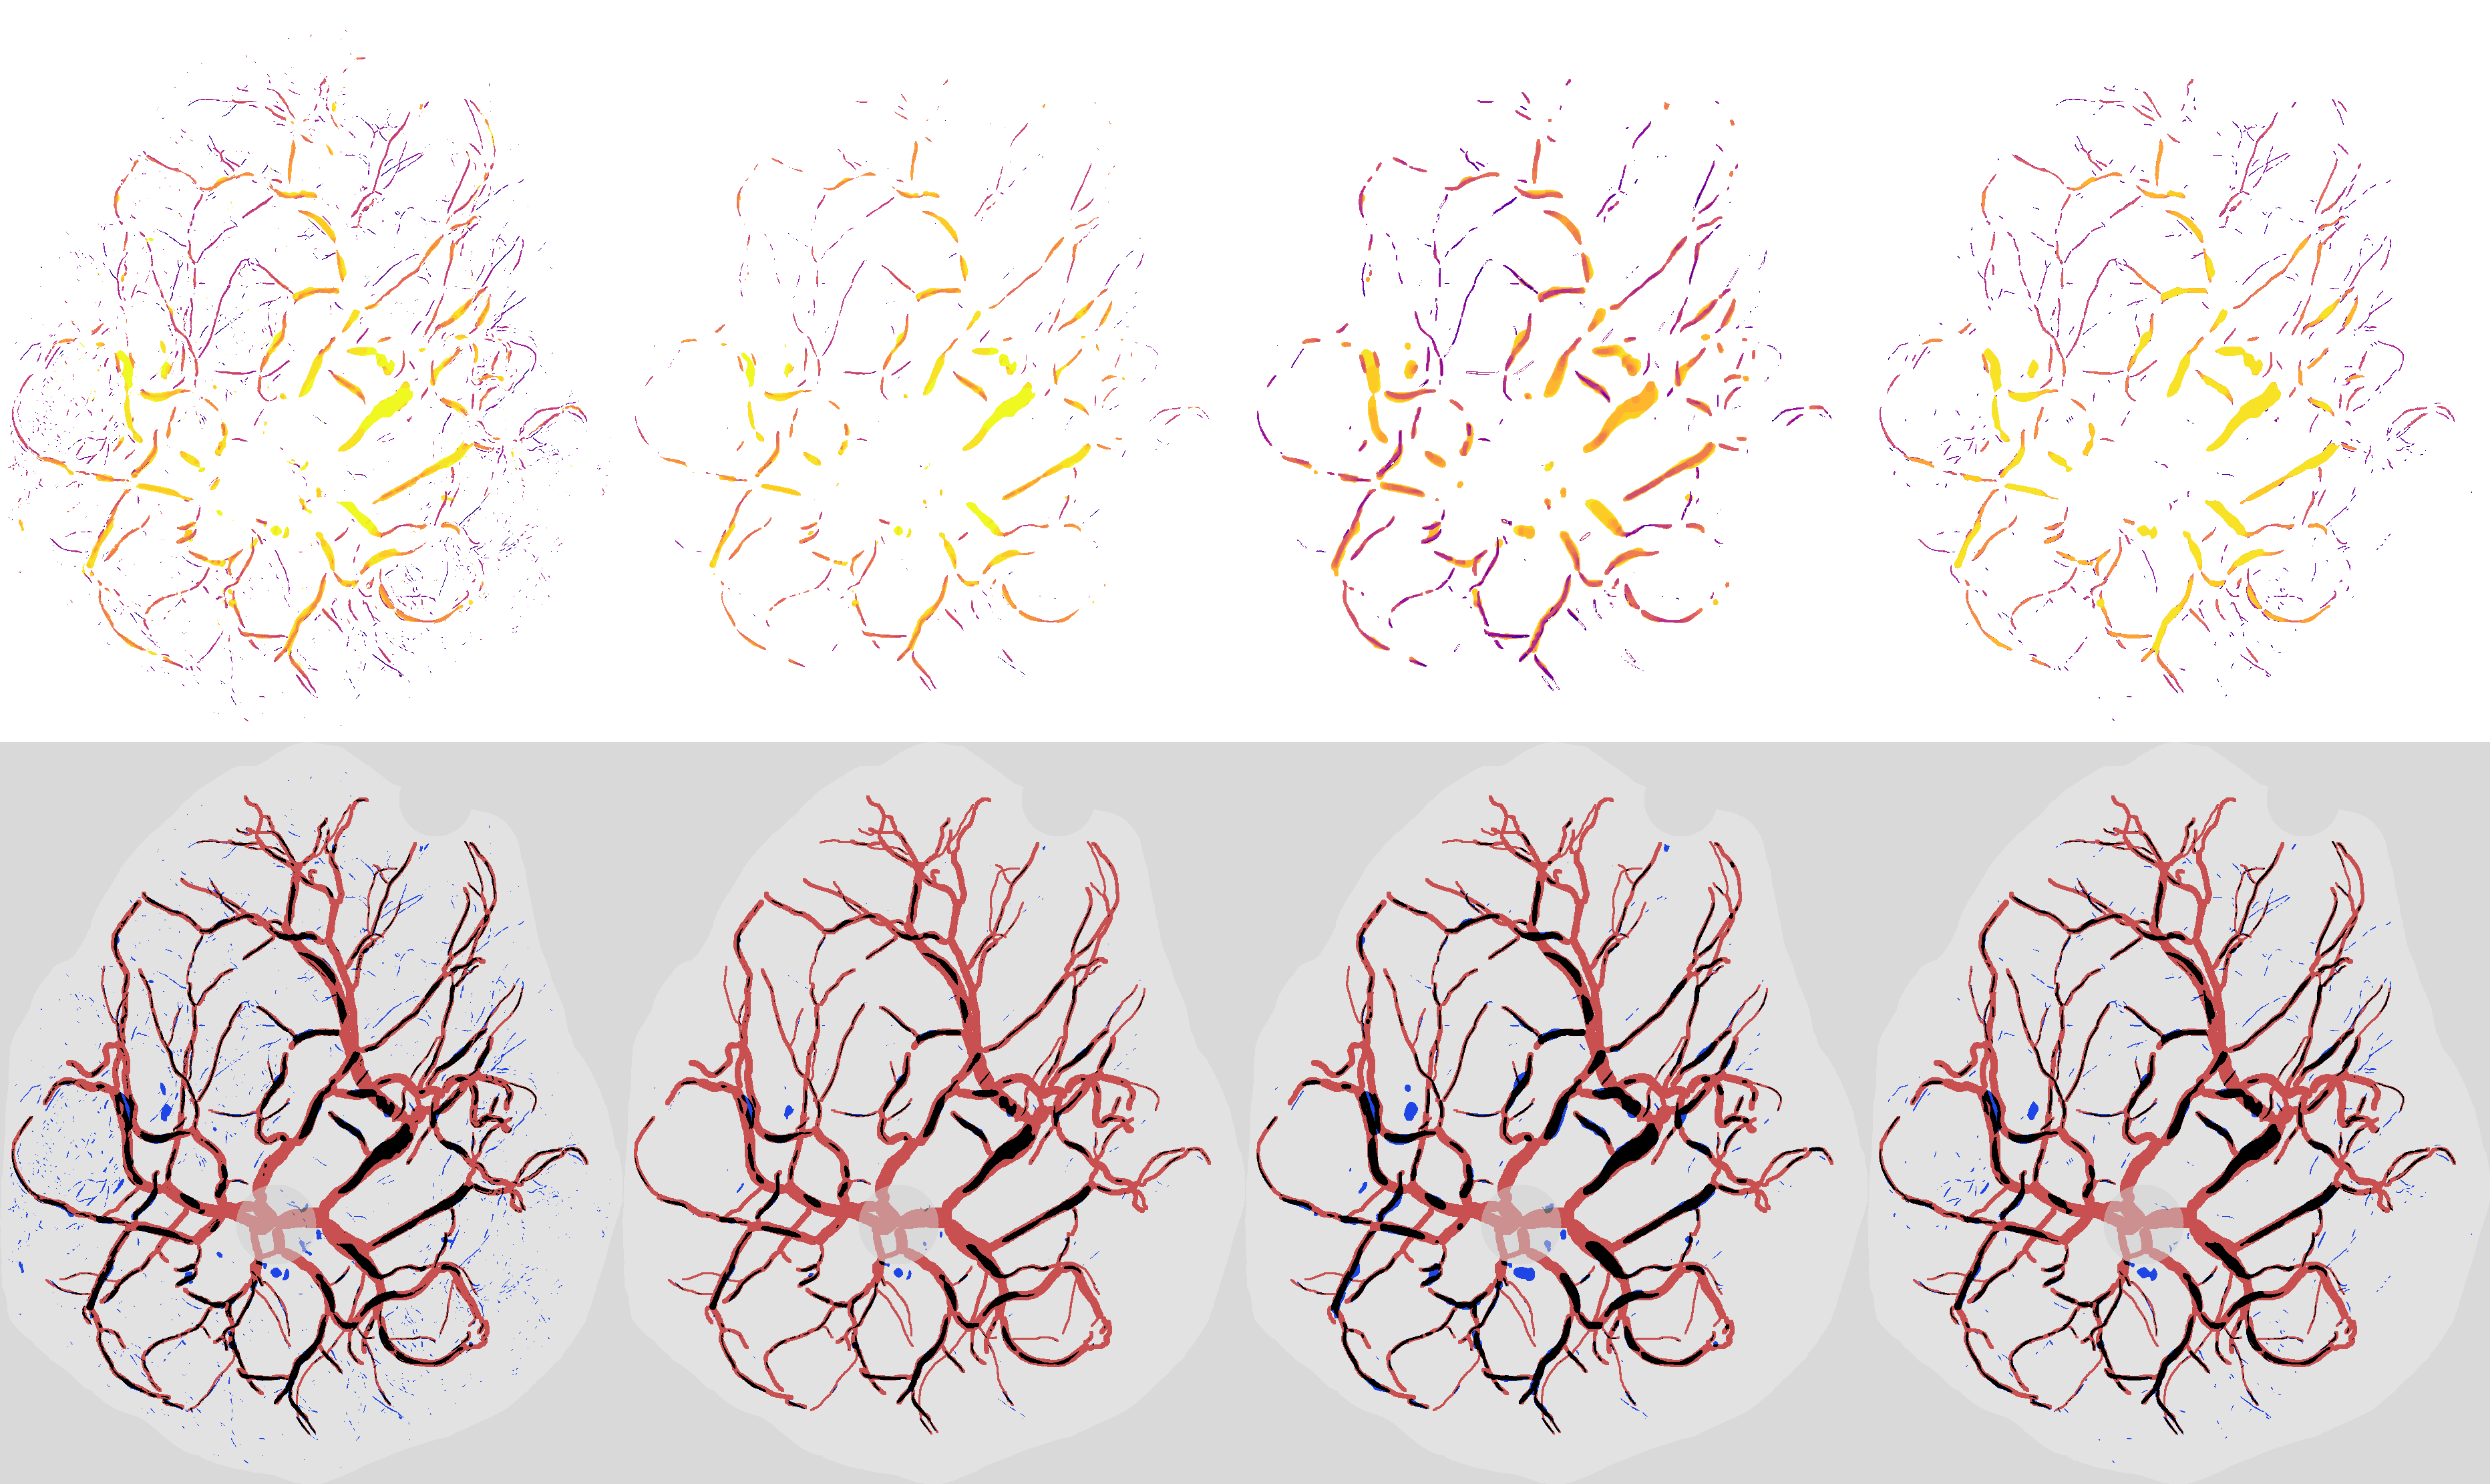
\includegraphics[width=\linewidth]{M2-T-BN2050224}
%	\caption{Sample of Frangi-based Segmentation Methods (pt. 2)}
%\end{figure}

%\begin{table}[p]\centering
%	\begin{tabular}{l|rrrr}
%		{} &        PF &        FA &        RW &        PS \\
%		\hline
%		MCC           &  0.4872 &  0.4208 &  0.5249 &  0.4877 \\
%		%\hline
%		skel coverage &  0.5085 &  0.3245 &  0.4493 &  0.4650 \\
%		%\hline
%		precision     &  0.8044 &  0.9472 &  0.8858 &  0.8697 \\
%	\end{tabular}
%	\caption{Scores for merging techniques}
%\end{table}:

\section{Variations in the Data Set and Imperfections of the Ground Truth} \label{sec:NCS-dataset-issues}
\begin{sidewaysfigure}
	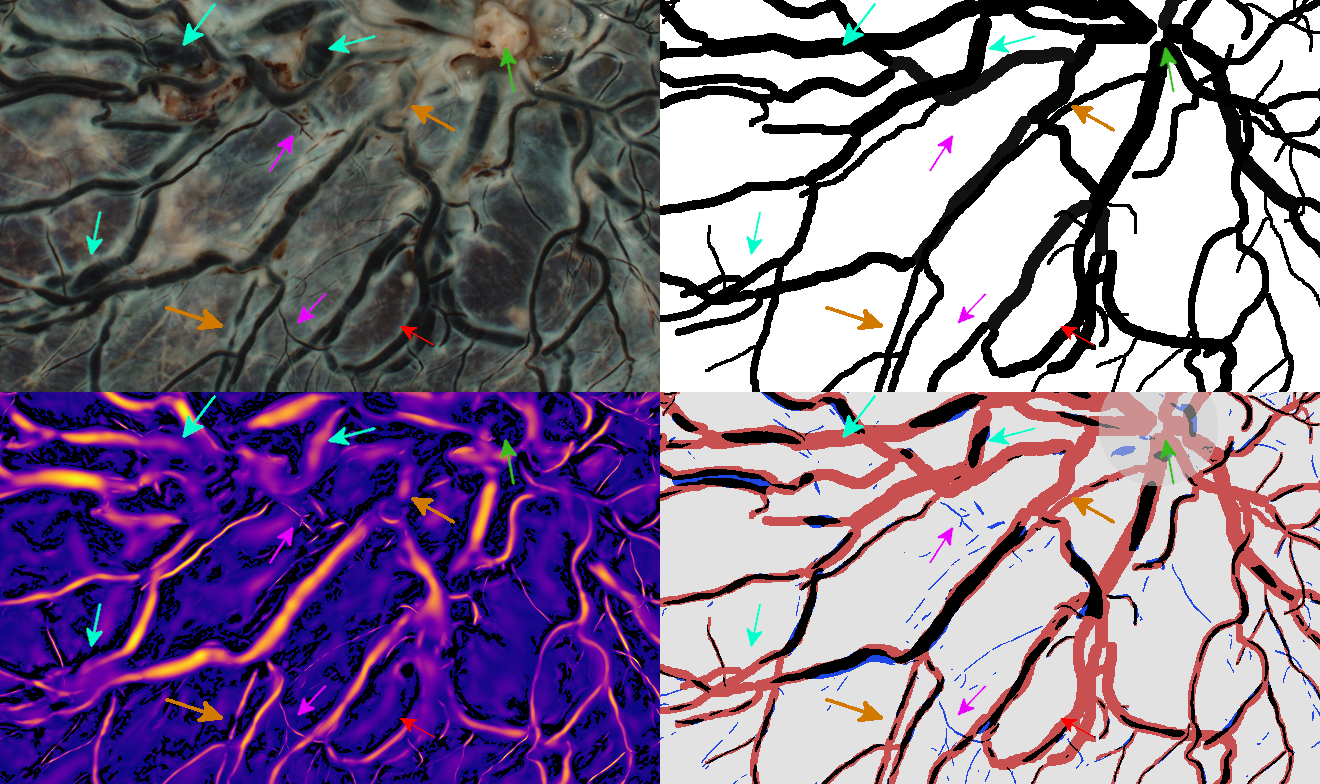
\includegraphics[width=\textwidth]{annotations-montage-2by2}
	\caption{Issues with the ground truth manifesting in Frangi vesselness scores}
	\label{fig:annotated-montage}
\end{sidewaysfigure}

We must first qualify binary classification. There are limitations intrinsic to the image domain and tracing protocol that make our ground truth tracing somewhat inaccurate. In \cref{fig:annotated-montage} we demonstrate a few common issues with the samples. The four figures show (top left) the original colored raw sample, (top right) the ground truth tracing, (bottom left) \Vmax, and (bottom right) the confusion matrix after some segmentation strategy. %"sieving strategy."
The green arrow points to the umbilical stump. You can see there is circular noise around this point, and in general perfusion around this point is very low--many of these vessels have been estimated by the tracer. The orange arrows represent points where perfusion is very low, perhaps caused by a clot in the blood vessel. The pink arrows point to vessels that were not traced, although they are clearly visible. The blue arrows point to where the shape of the vessel and the trace clearly do not agree. There any many more examples of these in the frame, and many more across all samples.
The red arrow points to an issue unrelated to the ground truth, but an issue that arise when selecting scales in our multiscale methodology-- this is a point of dark curvature that represents noise at larger scales. As you can see from the \Vmax of this inset, there is a positive response in this dead space between vessels, and there is another one that appears in the bottom left between two close vessels of similar size.

The sample we examined was a relatively well-behaved sample compared to others. Conversely, in \cref{fig:bad-gallery}, we give examples of some sampled that did not respond well to the Frangi filter, nor any of our Frangi-based segmentation methods. As can be seen from this gallery, poor perfusion of the blood vessels and large amounts of high constrast background is the common thread. One particular sample has very large arteries that were not reported. Increasing the scale size might fix the issue for this particular sample.

We have empirically identified a few reasons for issues. Although we have in many cases removed border areas from consideration where they would cause a large false response (see \cref{sec:boundary-dilation} for our discussion on boundary dilation), some samples still demonstrate noise around the ``collar'' of each plate. This can marginally be seen in \cref{fig:detailed_frangi_with_table_ex2}--there is a large Frangi response in the bottom left that was not removed, and thus shows up in each simple segmentation.


\begin{figure}[p]
	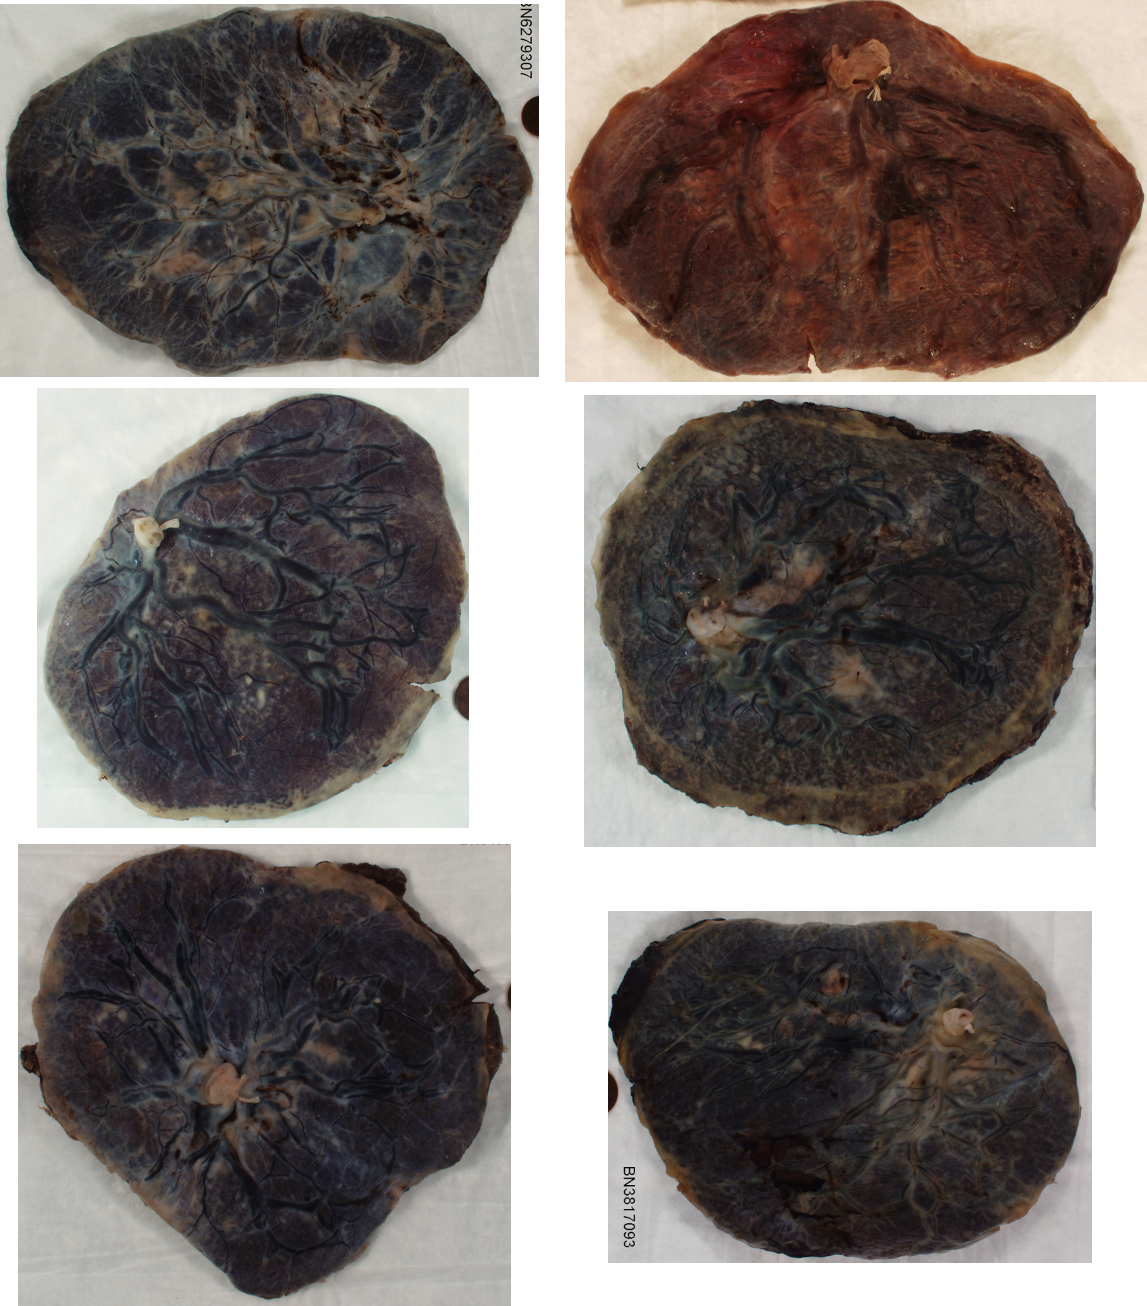
\includegraphics[width=\textwidth]{bad_gallery}
	\caption{Bad samples}
	\label{fig:bad-gallery}
\end{figure}

\section{Results}

In \cref{fig:compare_parameters_3by3_example1}, we demonstrate the usefulness of scricter parameters for the Frangi filter. Since the Frangi vesselness measure is a "probability-like" score, we should be interested--without doing any actual segmentation yet--to what extent this score aligns with the ground truth in a cumulative sense. We should hope at least that larger values of our vesselness measure should occur along vessels and not within the background. We define the cumulative vesselness ratio by ``integrating'' the max vesselness score over pixels in the ground truth and over the entire image and considering the ratio:

\begin{defn} The cumulative vesselness ratio for a particular parametrization of the multiscale Frangi filter is given by
	\begin{equation}
	CVR\left(\Vmax\right) := \frac{\sum_{G\subset\img} \Vmax(x_0, y_0)}{\sum_{\img} \Vmax(x_0,y_0)}
	\end{equation}
	where the sums on top and bottom are being carried out for all pixels $(x_0,y_0)$ in the "ground truth" subset $G$ in the image $\img$
	and over the entire image $\img$ itself, respectively.
\end{defn}

\cref{fig:compare_parameters_3by3_example1} and \cref{fig:compare_parameters_3by3_example2} show $\Vmax$ for two well-behaved samples with reported $CVR$. We see in both cases that stricter parameters (smaller $\beta$ and larger $\gamma$) correspond to an increased $CVR$. Each of these sample was run over the same scales (logarithmically spaced from $2^{-1.5}$ to $2^{3.5}$ with $N=20$ and the color output of each $\Vmax$ is normalized between 0 and 1.

% THESE ARE VERY GOOD BUT I PREFER THE LATER ONES, SINCE THEY HAVE MORE DEPTH
%\begin{figure}[p]\centering
%	\subfloat{
%		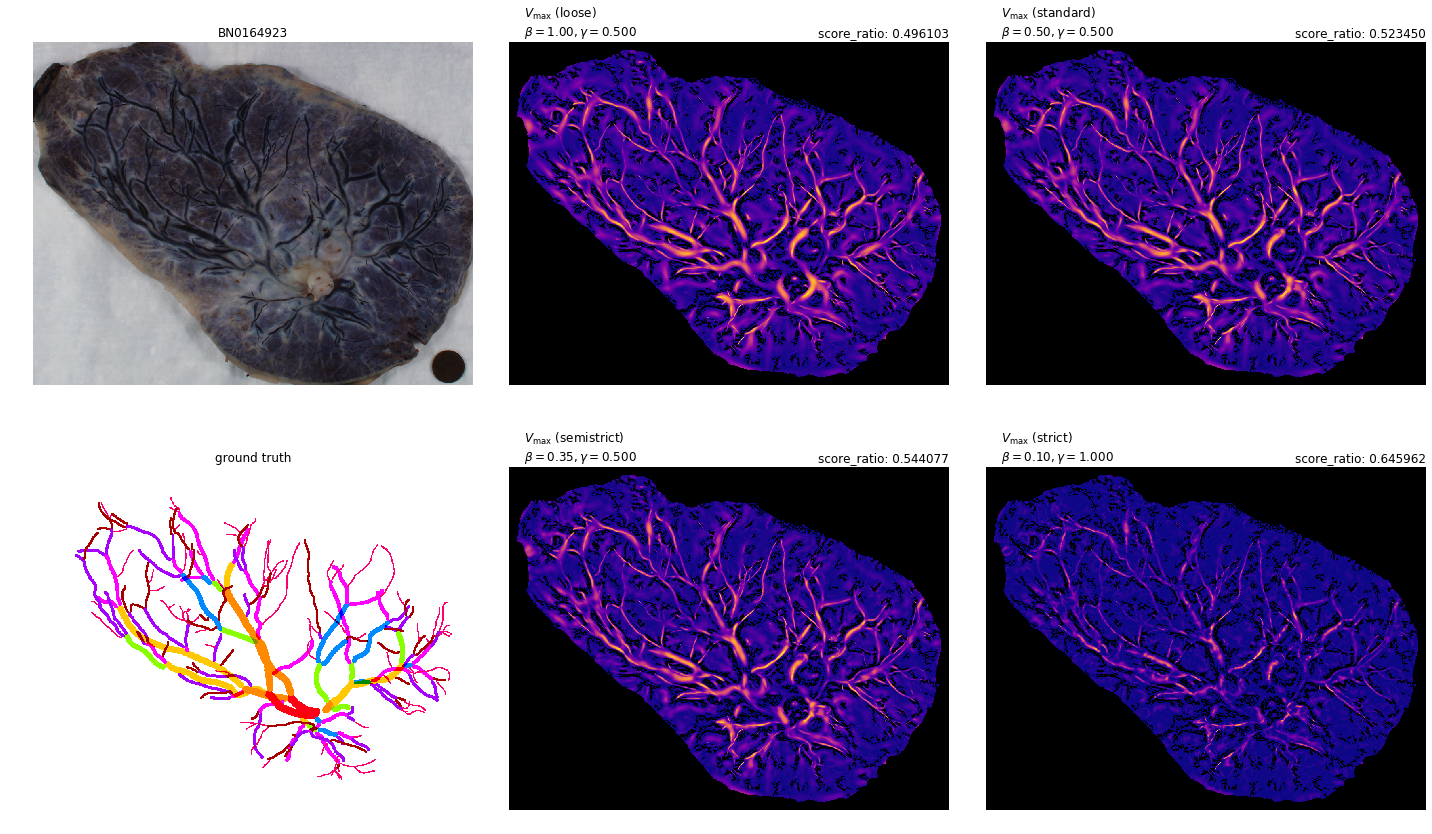
\includegraphics[width=\textwidth]{compare_parameters_BN0164923}
%	}\\
%	\subfloat{
%		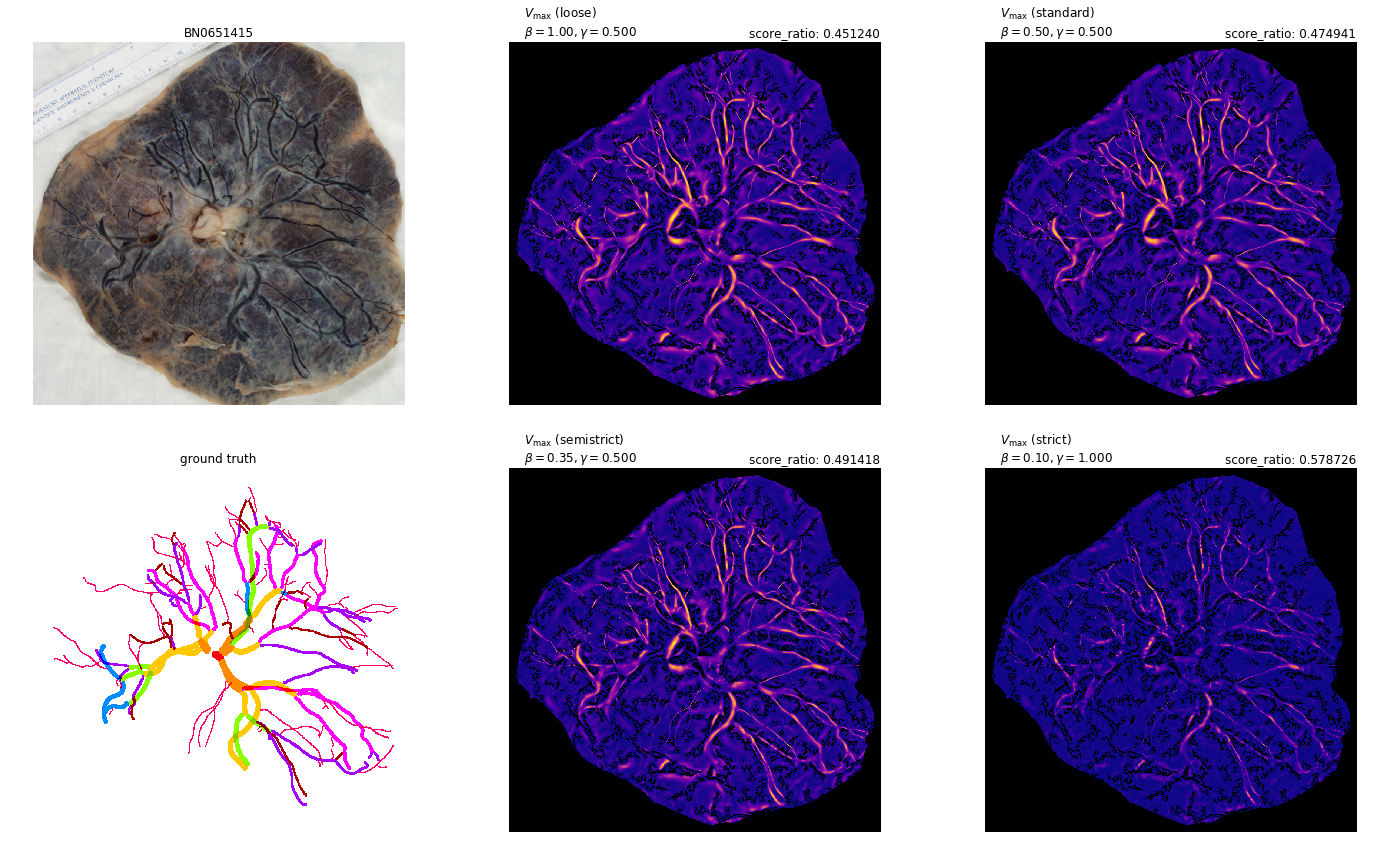
\includegraphics[width=\textwidth]{compare_parameters_BN0651415}
%	}
%	\caption{\Vmax  and $CVR$ for different parameter choices}
%	\label{fig:compare_parameters}
%\end{figure}



\begin{figure}[p]\centering
		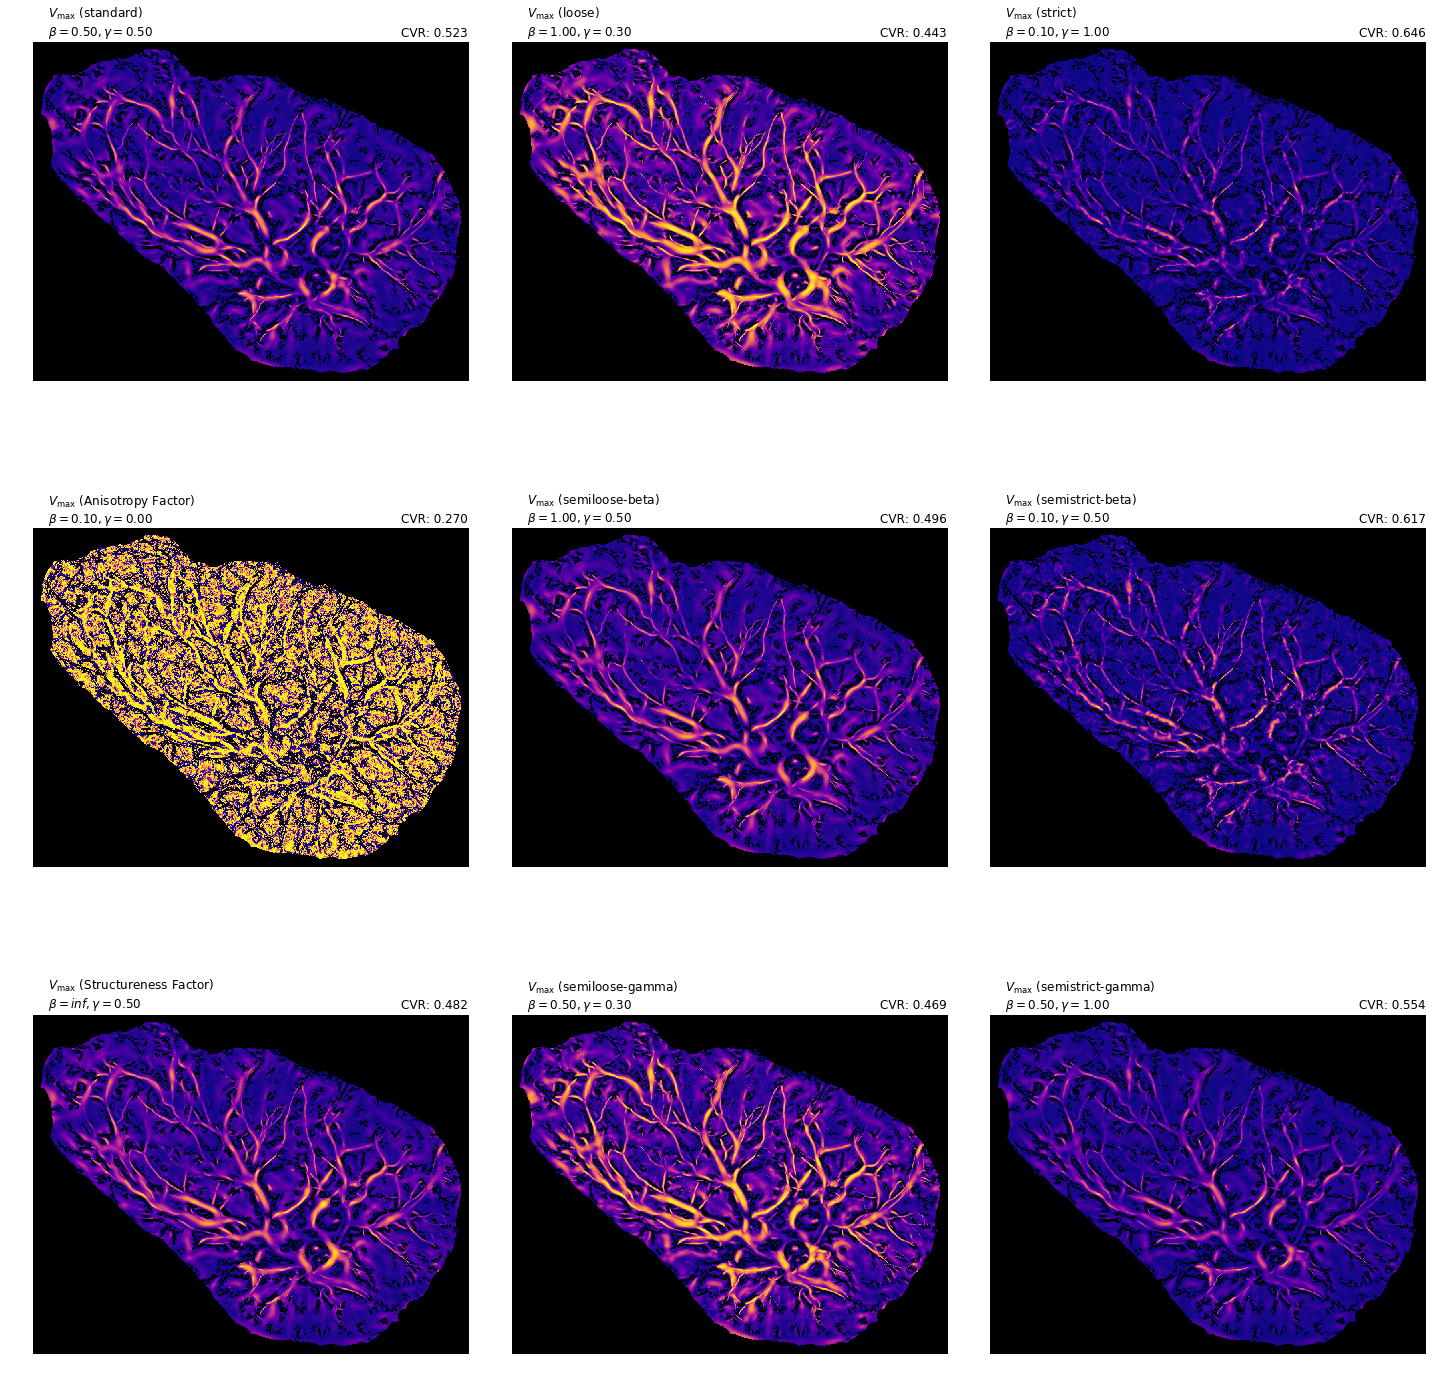
\includegraphics[width=\textwidth]{compare_parameters_3by3_example1}
	\caption{\Vmax  and $CVR$ for varying multiscale Frangi parametrizations (Example 1)}
	\label{fig:compare_parameters_3by3_example1}
\end{figure}

\begin{figure}[p]\centering
	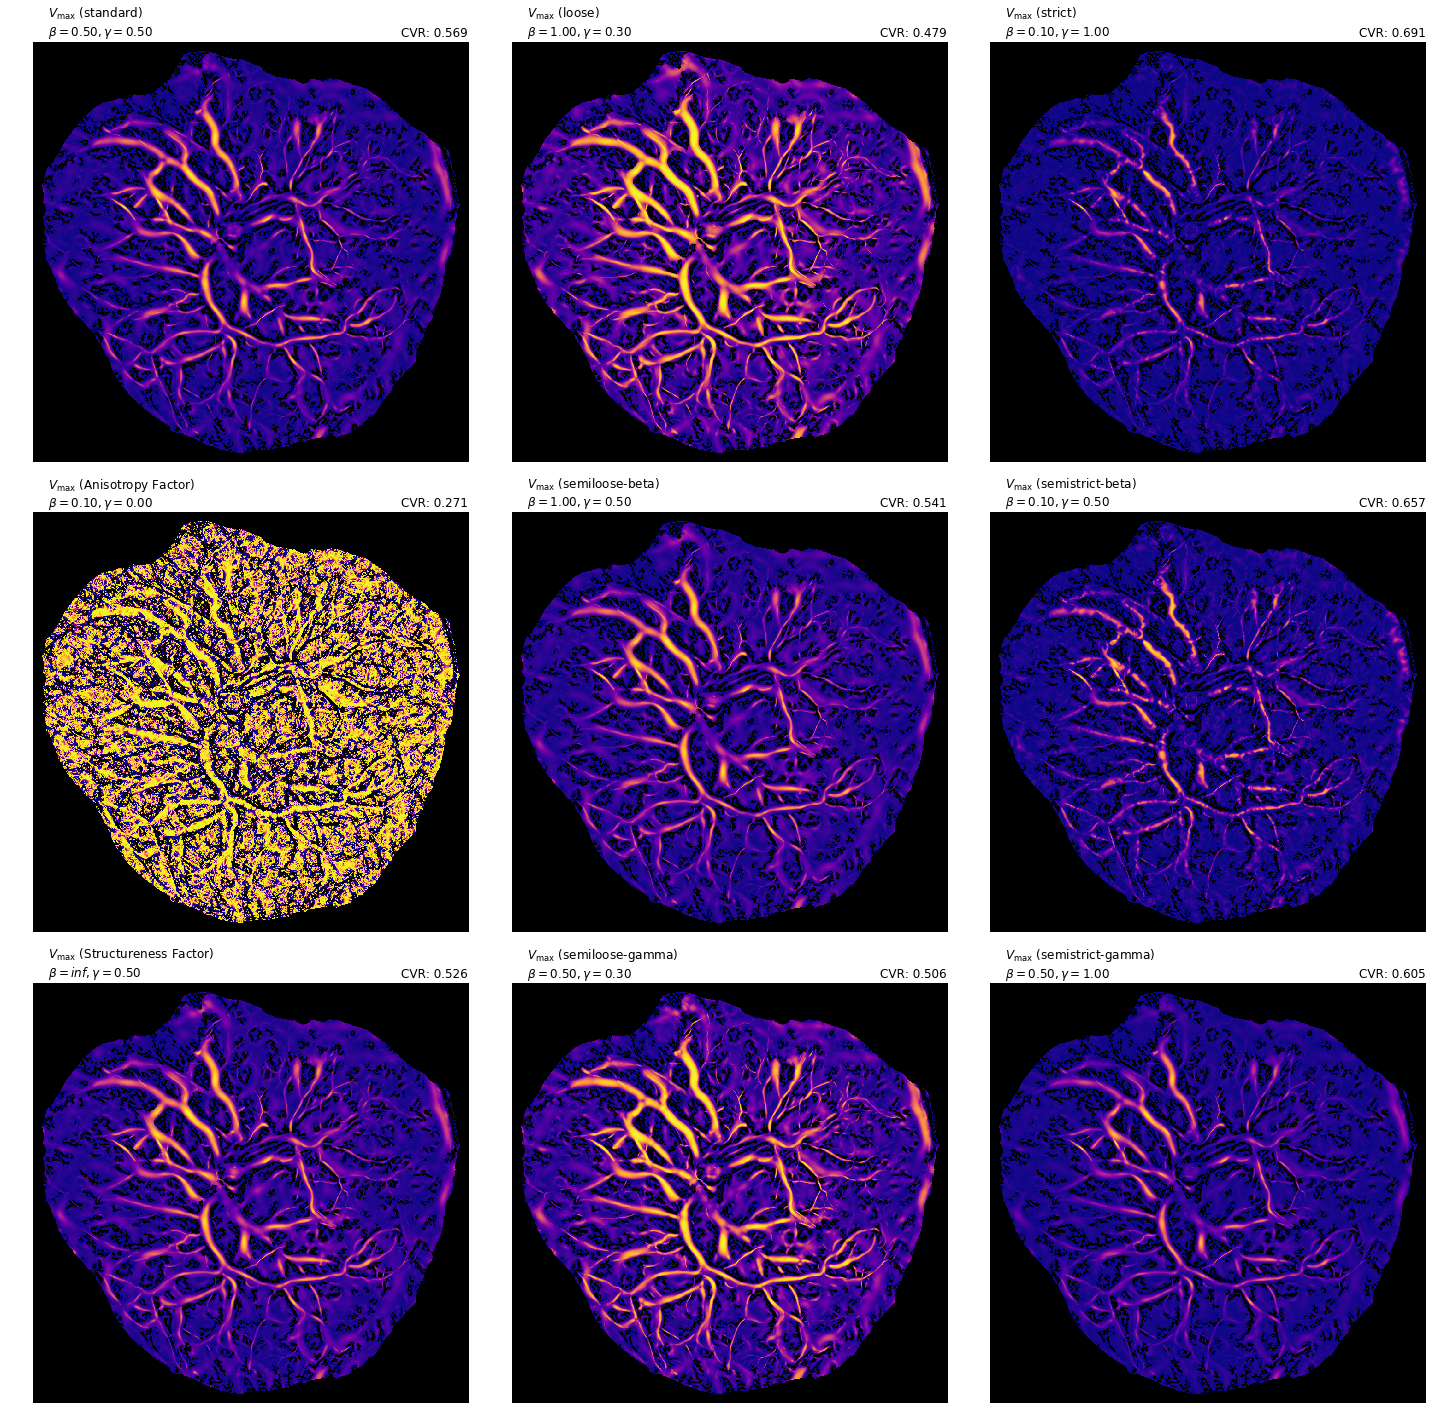
\includegraphics[width=\textwidth]{compare_parameters_3by3_example2}
	\caption{\Vmax  and $CVR$ for varying multiscale Frangi parametrizations (Example 2)}
	\label{fig:compare_parameters_3by3_example2}
\end{figure}

\begin{figure}\centering
	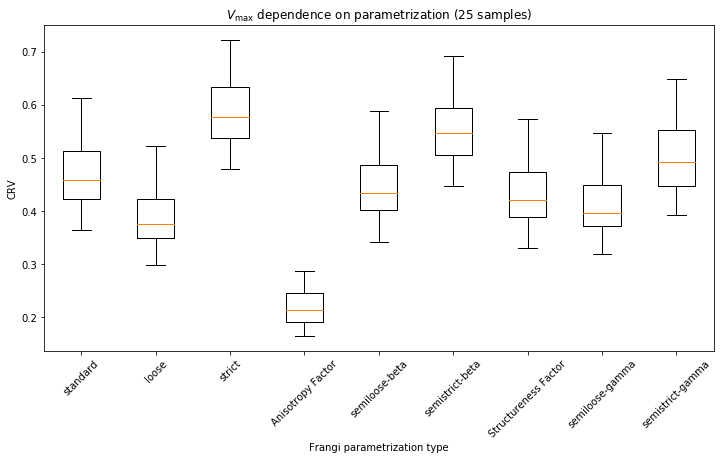
\includegraphics[width=\textwidth]{CRV_boxplot_quality0}
	\caption{$CVR$ scores of 25 samples under varying parametrizations}
  \label{fig:CVR-boxplot-quality0}
\end{figure}

In \cref{fig:CVR-boxplot-quality0} we show how the CVR is affected for 25 of the ``best'' samples, that is, those that generally fared better for segmentation techniques. This shows that the  results of \cref{fig:compare_parameters_3by3_example1} and \cref{fig:compare_parameters_3by3_example2} hold in general for all ``well-behaved'' samples in our image domain. 
\begin{figure}[p]\centering
  \subfloat{
  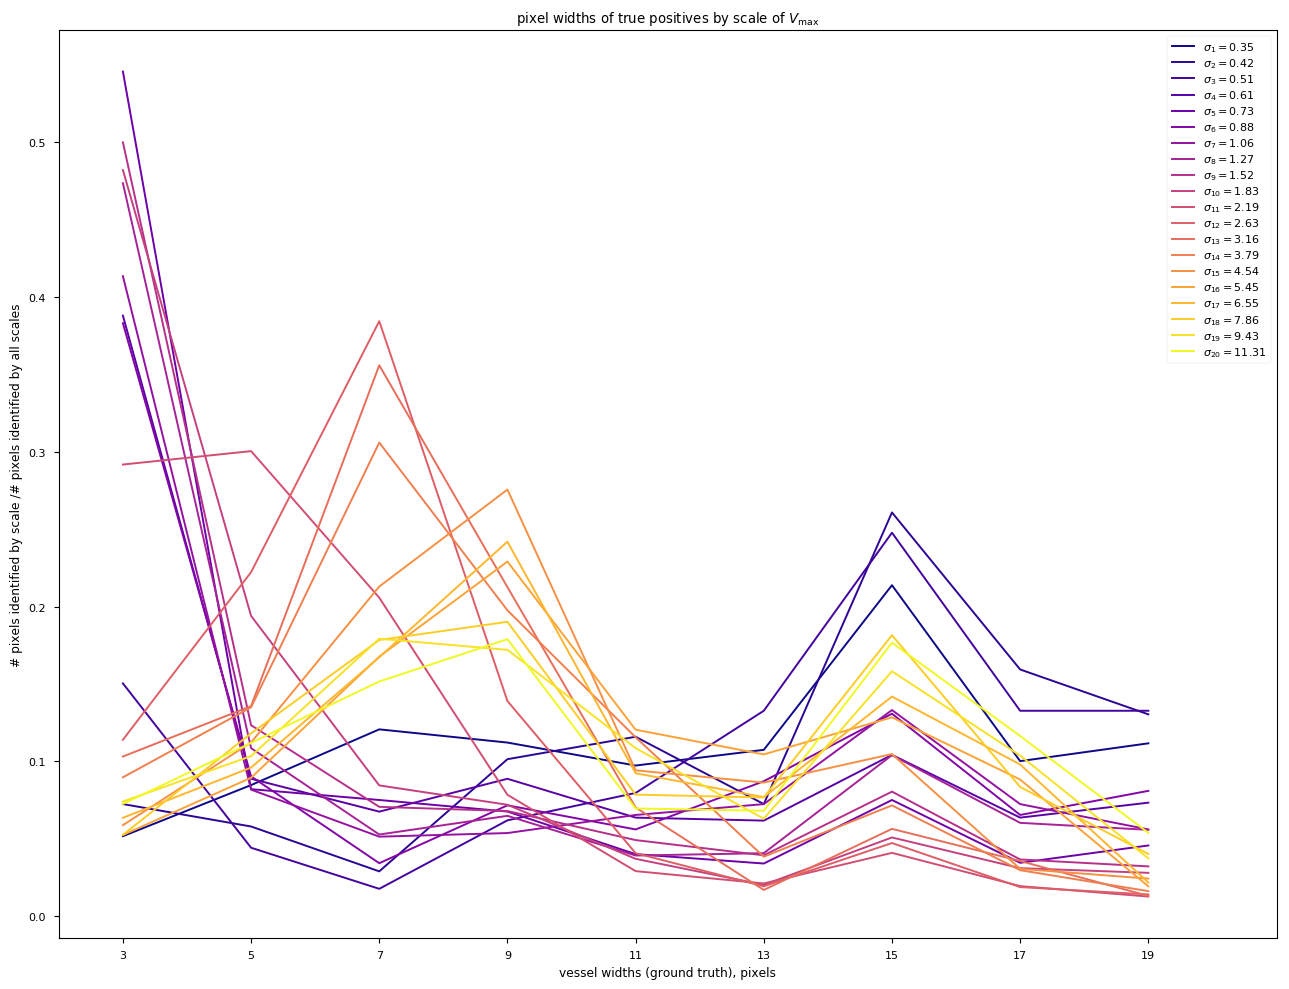
\includegraphics[width=0.85\textwidth]{Vmax_to_scale_normalized}
  }\\[-0.5cm]
  \subfloat{
  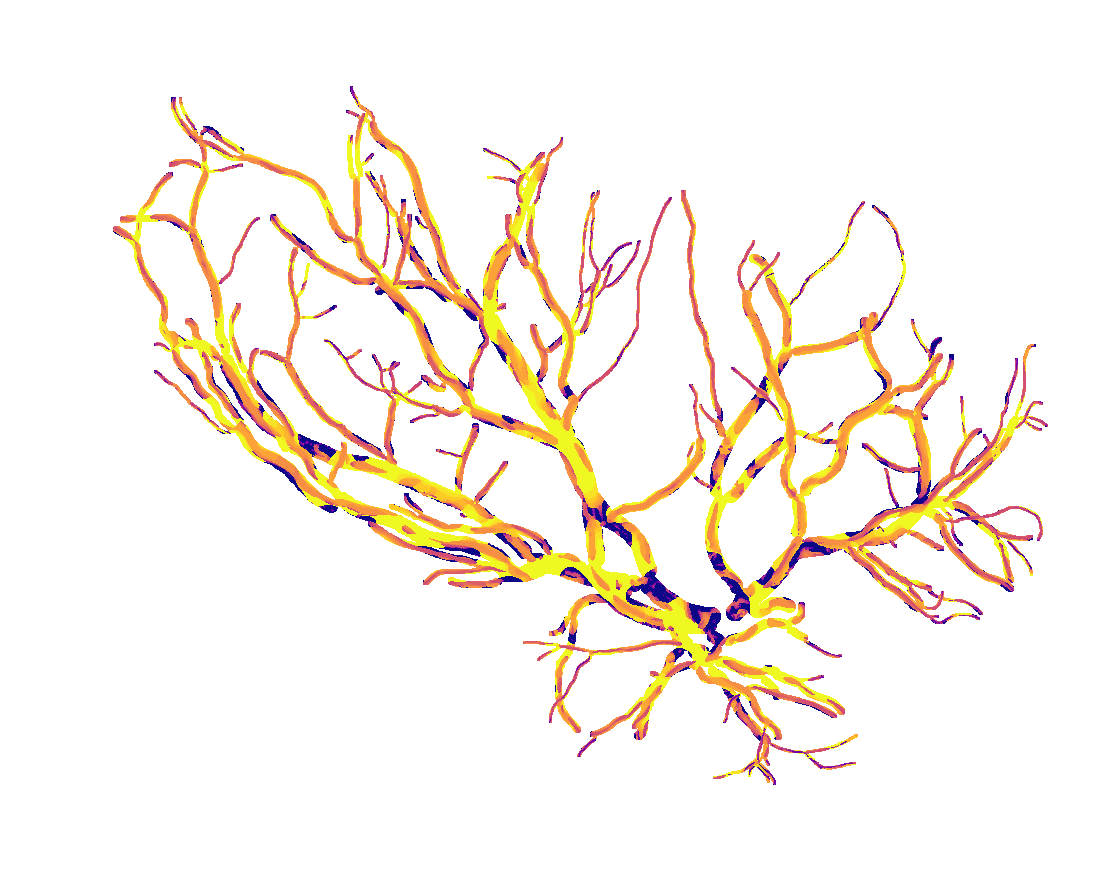
\includegraphics[width=0.85\textwidth]{frangi_argmax-trace}
  }
  \caption{Scale of maximum Frangi score for true positives and false negatives}
\end{figure}

\begin{figure}[p]\centering
  \subfloat{
    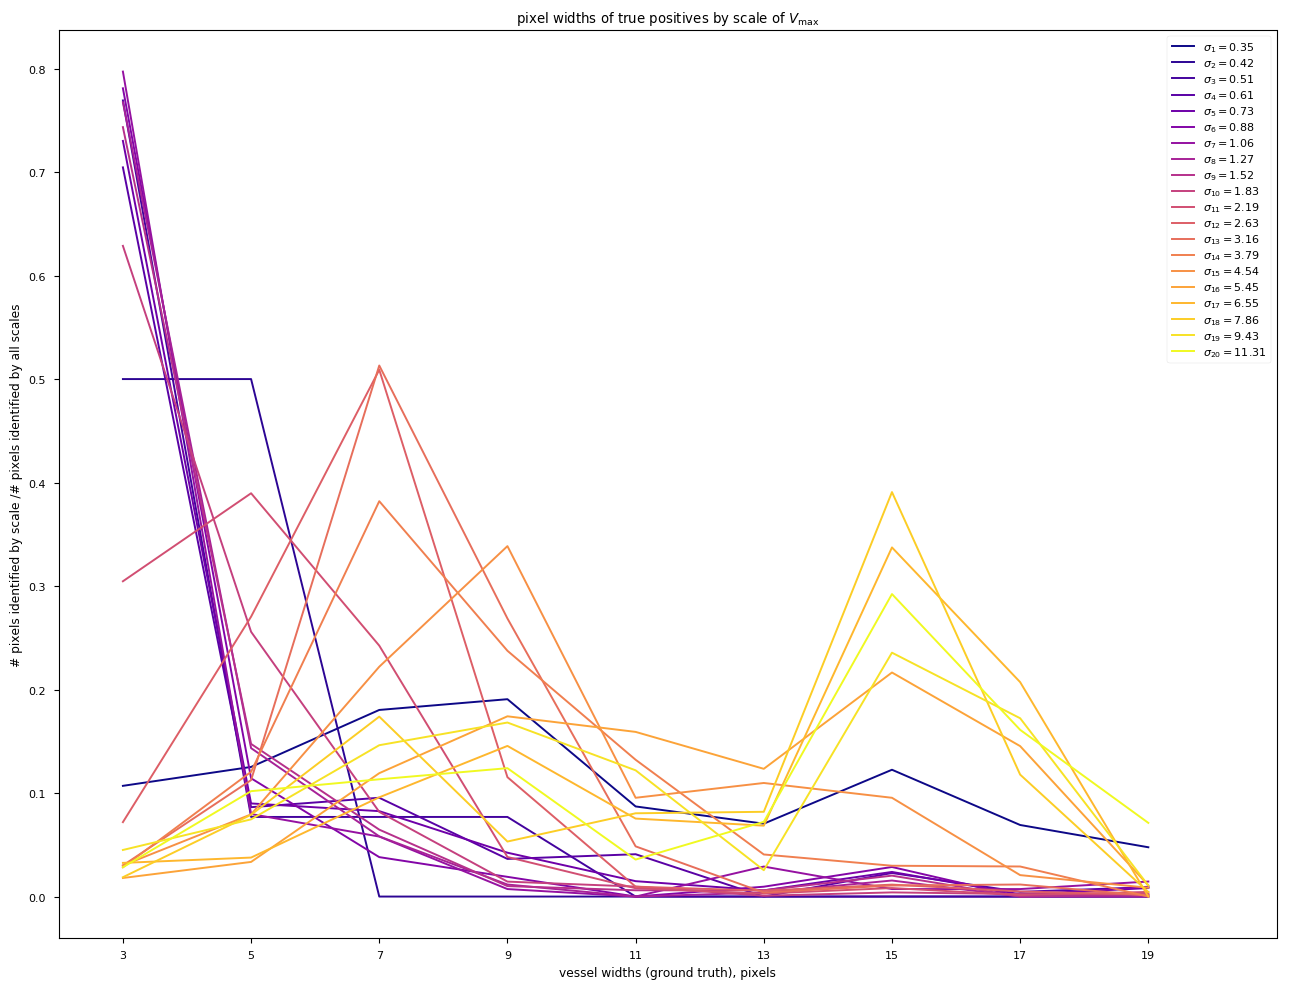
\includegraphics[width=0.85\textwidth]{Vmax_to_scale_normalized_with_approx}
  }\\[-0.5cm]
  \subfloat{
    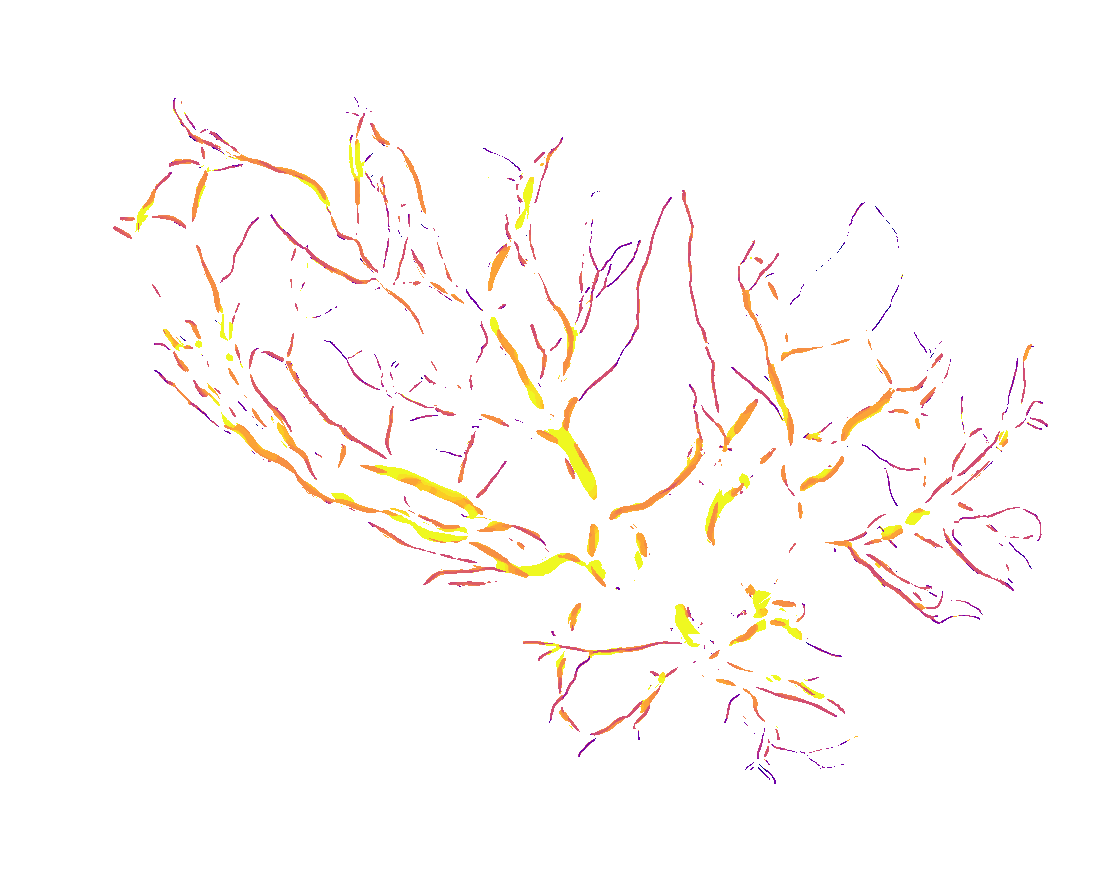
\includegraphics[width=0.85\textwidth]{frangi_argmax-trace-approx}
  }
  \caption{Scale of maximum Frangi score for true positives only (percentile filtering)}
\end{figure}

\begin{figure}[p]
  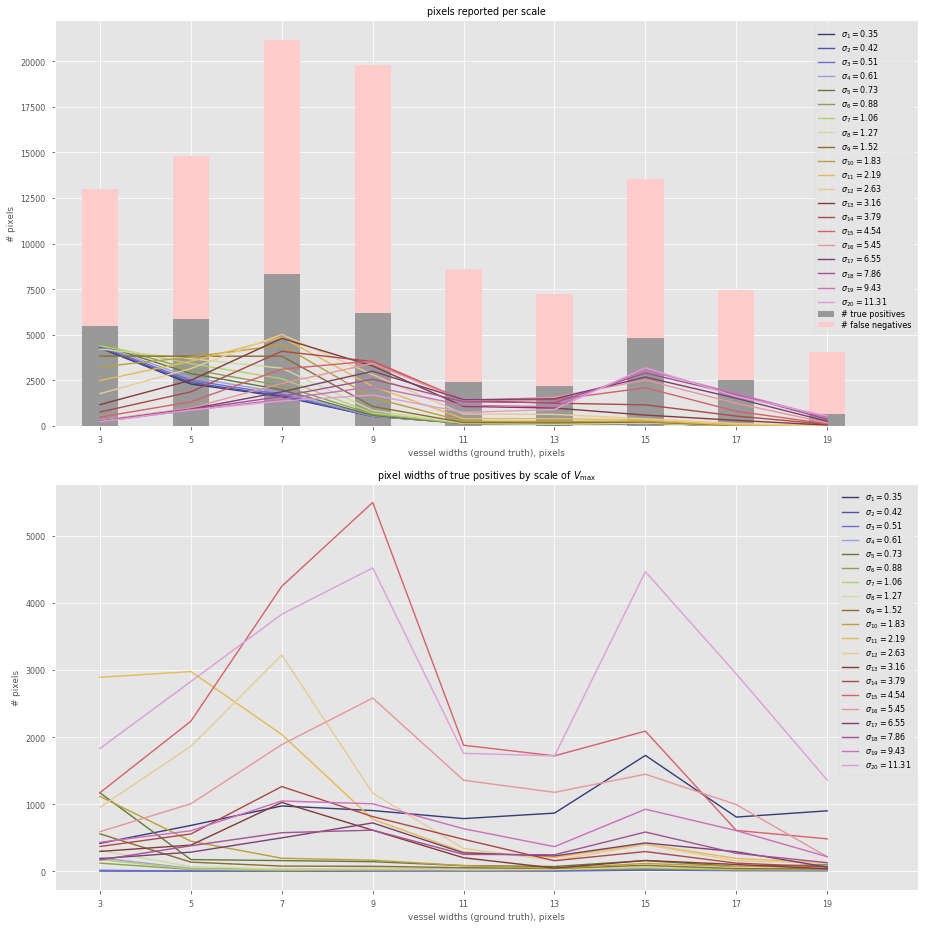
\includegraphics[width=\textwidth]{test-scale-width}
  \caption{Pixel Width of Ground Truth vs. Scale Length for True Positives}
\end{figure}
